% Options for packages loaded elsewhere
\PassOptionsToPackage{unicode}{hyperref}
\PassOptionsToPackage{hyphens}{url}
\PassOptionsToPackage{dvipsnames,svgnames,x11names}{xcolor}
%
\documentclass[
  letterpaper,
  DIV=11,
  numbers=noendperiod]{scrreprt}

\usepackage{amsmath,amssymb}
\usepackage{lmodern}
\usepackage{iftex}
\ifPDFTeX
  \usepackage[T1]{fontenc}
  \usepackage[utf8]{inputenc}
  \usepackage{textcomp} % provide euro and other symbols
\else % if luatex or xetex
  \usepackage{unicode-math}
  \defaultfontfeatures{Scale=MatchLowercase}
  \defaultfontfeatures[\rmfamily]{Ligatures=TeX,Scale=1}
\fi
% Use upquote if available, for straight quotes in verbatim environments
\IfFileExists{upquote.sty}{\usepackage{upquote}}{}
\IfFileExists{microtype.sty}{% use microtype if available
  \usepackage[]{microtype}
  \UseMicrotypeSet[protrusion]{basicmath} % disable protrusion for tt fonts
}{}
\makeatletter
\@ifundefined{KOMAClassName}{% if non-KOMA class
  \IfFileExists{parskip.sty}{%
    \usepackage{parskip}
  }{% else
    \setlength{\parindent}{0pt}
    \setlength{\parskip}{6pt plus 2pt minus 1pt}}
}{% if KOMA class
  \KOMAoptions{parskip=half}}
\makeatother
\usepackage{xcolor}
\setlength{\emergencystretch}{3em} % prevent overfull lines
\setcounter{secnumdepth}{5}
% Make \paragraph and \subparagraph free-standing
\ifx\paragraph\undefined\else
  \let\oldparagraph\paragraph
  \renewcommand{\paragraph}[1]{\oldparagraph{#1}\mbox{}}
\fi
\ifx\subparagraph\undefined\else
  \let\oldsubparagraph\subparagraph
  \renewcommand{\subparagraph}[1]{\oldsubparagraph{#1}\mbox{}}
\fi

\usepackage{color}
\usepackage{fancyvrb}
\newcommand{\VerbBar}{|}
\newcommand{\VERB}{\Verb[commandchars=\\\{\}]}
\DefineVerbatimEnvironment{Highlighting}{Verbatim}{commandchars=\\\{\}}
% Add ',fontsize=\small' for more characters per line
\usepackage{framed}
\definecolor{shadecolor}{RGB}{241,243,245}
\newenvironment{Shaded}{\begin{snugshade}}{\end{snugshade}}
\newcommand{\AlertTok}[1]{\textcolor[rgb]{0.68,0.00,0.00}{#1}}
\newcommand{\AnnotationTok}[1]{\textcolor[rgb]{0.37,0.37,0.37}{#1}}
\newcommand{\AttributeTok}[1]{\textcolor[rgb]{0.40,0.45,0.13}{#1}}
\newcommand{\BaseNTok}[1]{\textcolor[rgb]{0.68,0.00,0.00}{#1}}
\newcommand{\BuiltInTok}[1]{\textcolor[rgb]{0.00,0.23,0.31}{#1}}
\newcommand{\CharTok}[1]{\textcolor[rgb]{0.13,0.47,0.30}{#1}}
\newcommand{\CommentTok}[1]{\textcolor[rgb]{0.37,0.37,0.37}{#1}}
\newcommand{\CommentVarTok}[1]{\textcolor[rgb]{0.37,0.37,0.37}{\textit{#1}}}
\newcommand{\ConstantTok}[1]{\textcolor[rgb]{0.56,0.35,0.01}{#1}}
\newcommand{\ControlFlowTok}[1]{\textcolor[rgb]{0.00,0.23,0.31}{#1}}
\newcommand{\DataTypeTok}[1]{\textcolor[rgb]{0.68,0.00,0.00}{#1}}
\newcommand{\DecValTok}[1]{\textcolor[rgb]{0.68,0.00,0.00}{#1}}
\newcommand{\DocumentationTok}[1]{\textcolor[rgb]{0.37,0.37,0.37}{\textit{#1}}}
\newcommand{\ErrorTok}[1]{\textcolor[rgb]{0.68,0.00,0.00}{#1}}
\newcommand{\ExtensionTok}[1]{\textcolor[rgb]{0.00,0.23,0.31}{#1}}
\newcommand{\FloatTok}[1]{\textcolor[rgb]{0.68,0.00,0.00}{#1}}
\newcommand{\FunctionTok}[1]{\textcolor[rgb]{0.28,0.35,0.67}{#1}}
\newcommand{\ImportTok}[1]{\textcolor[rgb]{0.00,0.46,0.62}{#1}}
\newcommand{\InformationTok}[1]{\textcolor[rgb]{0.37,0.37,0.37}{#1}}
\newcommand{\KeywordTok}[1]{\textcolor[rgb]{0.00,0.23,0.31}{#1}}
\newcommand{\NormalTok}[1]{\textcolor[rgb]{0.00,0.23,0.31}{#1}}
\newcommand{\OperatorTok}[1]{\textcolor[rgb]{0.37,0.37,0.37}{#1}}
\newcommand{\OtherTok}[1]{\textcolor[rgb]{0.00,0.23,0.31}{#1}}
\newcommand{\PreprocessorTok}[1]{\textcolor[rgb]{0.68,0.00,0.00}{#1}}
\newcommand{\RegionMarkerTok}[1]{\textcolor[rgb]{0.00,0.23,0.31}{#1}}
\newcommand{\SpecialCharTok}[1]{\textcolor[rgb]{0.37,0.37,0.37}{#1}}
\newcommand{\SpecialStringTok}[1]{\textcolor[rgb]{0.13,0.47,0.30}{#1}}
\newcommand{\StringTok}[1]{\textcolor[rgb]{0.13,0.47,0.30}{#1}}
\newcommand{\VariableTok}[1]{\textcolor[rgb]{0.07,0.07,0.07}{#1}}
\newcommand{\VerbatimStringTok}[1]{\textcolor[rgb]{0.13,0.47,0.30}{#1}}
\newcommand{\WarningTok}[1]{\textcolor[rgb]{0.37,0.37,0.37}{\textit{#1}}}

\providecommand{\tightlist}{%
  \setlength{\itemsep}{0pt}\setlength{\parskip}{0pt}}\usepackage{longtable,booktabs,array}
\usepackage{calc} % for calculating minipage widths
% Correct order of tables after \paragraph or \subparagraph
\usepackage{etoolbox}
\makeatletter
\patchcmd\longtable{\par}{\if@noskipsec\mbox{}\fi\par}{}{}
\makeatother
% Allow footnotes in longtable head/foot
\IfFileExists{footnotehyper.sty}{\usepackage{footnotehyper}}{\usepackage{footnote}}
\makesavenoteenv{longtable}
\usepackage{graphicx}
\makeatletter
\def\maxwidth{\ifdim\Gin@nat@width>\linewidth\linewidth\else\Gin@nat@width\fi}
\def\maxheight{\ifdim\Gin@nat@height>\textheight\textheight\else\Gin@nat@height\fi}
\makeatother
% Scale images if necessary, so that they will not overflow the page
% margins by default, and it is still possible to overwrite the defaults
% using explicit options in \includegraphics[width, height, ...]{}
\setkeys{Gin}{width=\maxwidth,height=\maxheight,keepaspectratio}
% Set default figure placement to htbp
\makeatletter
\def\fps@figure{htbp}
\makeatother
\newlength{\cslhangindent}
\setlength{\cslhangindent}{1.5em}
\newlength{\csllabelwidth}
\setlength{\csllabelwidth}{3em}
\newlength{\cslentryspacingunit} % times entry-spacing
\setlength{\cslentryspacingunit}{\parskip}
\newenvironment{CSLReferences}[2] % #1 hanging-ident, #2 entry spacing
 {% don't indent paragraphs
  \setlength{\parindent}{0pt}
  % turn on hanging indent if param 1 is 1
  \ifodd #1
  \let\oldpar\par
  \def\par{\hangindent=\cslhangindent\oldpar}
  \fi
  % set entry spacing
  \setlength{\parskip}{#2\cslentryspacingunit}
 }%
 {}
\usepackage{calc}
\newcommand{\CSLBlock}[1]{#1\hfill\break}
\newcommand{\CSLLeftMargin}[1]{\parbox[t]{\csllabelwidth}{#1}}
\newcommand{\CSLRightInline}[1]{\parbox[t]{\linewidth - \csllabelwidth}{#1}\break}
\newcommand{\CSLIndent}[1]{\hspace{\cslhangindent}#1}

<script src="site_libs/htmlwidgets-1.6.0/htmlwidgets.js"></script>
<script src="site_libs/viz-1.8.2/viz.js"></script>
<link href="site_libs/DiagrammeR-styles-0.2/styles.css" rel="stylesheet" />
<script src="site_libs/grViz-binding-1.0.9/grViz.js"></script>
\KOMAoption{captions}{tableheading}
\makeatletter
\@ifpackageloaded{tcolorbox}{}{\usepackage[many]{tcolorbox}}
\@ifpackageloaded{fontawesome5}{}{\usepackage{fontawesome5}}
\definecolor{quarto-callout-color}{HTML}{909090}
\definecolor{quarto-callout-note-color}{HTML}{0758E5}
\definecolor{quarto-callout-important-color}{HTML}{CC1914}
\definecolor{quarto-callout-warning-color}{HTML}{EB9113}
\definecolor{quarto-callout-tip-color}{HTML}{00A047}
\definecolor{quarto-callout-caution-color}{HTML}{FC5300}
\definecolor{quarto-callout-color-frame}{HTML}{acacac}
\definecolor{quarto-callout-note-color-frame}{HTML}{4582ec}
\definecolor{quarto-callout-important-color-frame}{HTML}{d9534f}
\definecolor{quarto-callout-warning-color-frame}{HTML}{f0ad4e}
\definecolor{quarto-callout-tip-color-frame}{HTML}{02b875}
\definecolor{quarto-callout-caution-color-frame}{HTML}{fd7e14}
\makeatother
\makeatletter
\makeatother
\makeatletter
\@ifpackageloaded{bookmark}{}{\usepackage{bookmark}}
\makeatother
\makeatletter
\@ifpackageloaded{caption}{}{\usepackage{caption}}
\AtBeginDocument{%
\ifdefined\contentsname
  \renewcommand*\contentsname{Table of contents}
\else
  \newcommand\contentsname{Table of contents}
\fi
\ifdefined\listfigurename
  \renewcommand*\listfigurename{List of Figures}
\else
  \newcommand\listfigurename{List of Figures}
\fi
\ifdefined\listtablename
  \renewcommand*\listtablename{List of Tables}
\else
  \newcommand\listtablename{List of Tables}
\fi
\ifdefined\figurename
  \renewcommand*\figurename{Figure}
\else
  \newcommand\figurename{Figure}
\fi
\ifdefined\tablename
  \renewcommand*\tablename{Table}
\else
  \newcommand\tablename{Table}
\fi
}
\@ifpackageloaded{float}{}{\usepackage{float}}
\floatstyle{ruled}
\@ifundefined{c@chapter}{\newfloat{codelisting}{h}{lop}}{\newfloat{codelisting}{h}{lop}[chapter]}
\floatname{codelisting}{Listing}
\newcommand*\listoflistings{\listof{codelisting}{List of Listings}}
\makeatother
\makeatletter
\@ifpackageloaded{caption}{}{\usepackage{caption}}
\@ifpackageloaded{subcaption}{}{\usepackage{subcaption}}
\makeatother
\makeatletter
\@ifpackageloaded{tcolorbox}{}{\usepackage[many]{tcolorbox}}
\makeatother
\makeatletter
\@ifundefined{shadecolor}{\definecolor{shadecolor}{rgb}{.97, .97, .97}}
\makeatother
\makeatletter
\makeatother
\ifLuaTeX
  \usepackage{selnolig}  % disable illegal ligatures
\fi
\IfFileExists{bookmark.sty}{\usepackage{bookmark}}{\usepackage{hyperref}}
\IfFileExists{xurl.sty}{\usepackage{xurl}}{} % add URL line breaks if available
\urlstyle{same} % disable monospaced font for URLs
\hypersetup{
  pdftitle={Multilevel Thinking},
  pdfauthor={Andrew Grogan-Kaylor},
  colorlinks=true,
  linkcolor={blue},
  filecolor={Maroon},
  citecolor={Blue},
  urlcolor={Blue},
  pdfcreator={LaTeX via pandoc}}

\title{Multilevel Thinking}
\usepackage{etoolbox}
\makeatletter
\providecommand{\subtitle}[1]{% add subtitle to \maketitle
  \apptocmd{\@title}{\par {\large #1 \par}}{}{}
}
\makeatother
\subtitle{Using Multilevel Models To Thread The Needle Between
Universality and Cultural Specificity in Cross Cultural Research}
\author{Andrew Grogan-Kaylor}
\date{12/23/22}

\begin{document}
\maketitle
\ifdefined\Shaded\renewenvironment{Shaded}{\begin{tcolorbox}[boxrule=0pt, enhanced, borderline west={3pt}{0pt}{shadecolor}, frame hidden, sharp corners, interior hidden, breakable]}{\end{tcolorbox}}\fi

\renewcommand*\contentsname{Table of contents}
{
\hypersetup{linkcolor=}
\setcounter{tocdepth}{2}
\tableofcontents
}
\bookmarksetup{startatroot}

\hypertarget{the-usefulness-of-multilevel-modeling-and-multilevel-thinking}{%
\chapter{The Usefulness of Multilevel Modeling and Multilevel
Thinking}\label{the-usefulness-of-multilevel-modeling-and-multilevel-thinking}}

\begin{Shaded}
\begin{Highlighting}[]
\FunctionTok{library}\NormalTok{(ggplot2) }\CommentTok{\# beautiful graphs}

\FunctionTok{library}\NormalTok{(geomtextpath) }\CommentTok{\# path geoms}

\FunctionTok{library}\NormalTok{(dplyr) }\CommentTok{\# data wrangling}
\end{Highlighting}
\end{Shaded}

\begin{verbatim}

Attaching package: 'dplyr'
\end{verbatim}

\begin{verbatim}
The following objects are masked from 'package:stats':

    filter, lag
\end{verbatim}

\begin{verbatim}
The following objects are masked from 'package:base':

    intersect, setdiff, setequal, union
\end{verbatim}

\begin{Shaded}
\begin{Highlighting}[]
\FunctionTok{library}\NormalTok{(tidyr) }\CommentTok{\# data tidying}

\FunctionTok{library}\NormalTok{(pander) }\CommentTok{\# nice tables}

\CommentTok{\# library(gt) \# beautiful tables}

\FunctionTok{library}\NormalTok{(sf) }\CommentTok{\# simple (spatial) features}
\end{Highlighting}
\end{Shaded}

\begin{verbatim}
Linking to GEOS 3.10.2, GDAL 3.4.2, PROJ 8.2.1; sf_use_s2() is TRUE
\end{verbatim}

\begin{Shaded}
\begin{Highlighting}[]
\CommentTok{\# library(leaflet) \# beautiful maps}

\CommentTok{\# library(lme4) \# MLM}

\CommentTok{\# library(sjPlot) \# nice tables for MLM}

\FunctionTok{library}\NormalTok{(haven) }\CommentTok{\# read and write Stata}

\CommentTok{\# library(Statamarkdown) \# run Stata commands}

\FunctionTok{set.seed}\NormalTok{(}\DecValTok{3846}\NormalTok{) }\CommentTok{\# random seed}
\end{Highlighting}
\end{Shaded}

For decades now, multilevel models have been an important quantitative
tool for social research. While multilevel models have become ubiquitous
in social research, there are dimensions of these models that are
explored less frequently in published articles. This document arises
from my experiences of teaching a course entitled \emph{Multilevel and
Longitudinal Modeling} that I have taught for over a decade in the
\emph{Joint Doctoral Program in Social Work and Social Science} at the
University of Michigan.

My contention is that \emph{multilevel modeling} offers powerful tools
for understanding the \emph{multilevel data} that social researchers
often confront. For example, researchers are often interested in
studying outcomes for diverse groups of children in different schools,
residents of diverse and different neighborhoods, or individuals or
families living in diverse and different countries. Such inherently
multilevel data lead to analytic complexities, some of which appear to
me to be well understood, while others seem to be much less often
appreciated.

The point that I wish to make about multilevel data is that when
presented with complex multilevel data, failure to use the appropriate
multilevel model may lead to conclusions that are demonstrably
incorrect. Fortunately, many of these difficulties can be avoided with
applications of simple and straightforward multilevel models.

After presenting some initial ideas about multilevel modeling, I go on
to explore some more complex ideas about multilevel models that I see
less often in the published empirical literature. I focus especially on
the idea of \emph{multilevel models as the exploration of variation
across countries and cultures}.

Certainly, none of the statistical ideas contained in this document are
unique to me. There are thorough--and often much more mathematically
rigorous--presentations of many of the idea contained in this document
in some of the excellent foundational texts on multilevel modeling such
as the early book by Raudenbush \& Bryk (2002), the excellent book on
longitudinal models by Singer \& Willett (2003), and Rabe-Hesketh \&
Skrondal (2012)'s more recent and extremely comprehensive two volume
text. Luke (2004), and Kreft \& de Leeuw (1998), offer shorter, less
mathematical, but still excellent introductions to the topic of
multilevel modeling. Gelman et al. (2007) introduced me to the ideas
that in this document I describe as ``multilevel structure'' using an
example with voting patterns.

My intent in this document is to offer a kind of accessible tutorial for
applied researchers, including especially those who see their research
having some advocacy based component. My approach, while offering up
some equations, is less mathematical than some of the above mentioned
texts, and written with the intent of providing a clear and practically
focused guide for the applied researcher who is attempting to carry out
better research with diverse populations.

\bookmarksetup{startatroot}

\hypertarget{acknowledgements}{%
\chapter*{Acknowledgements}\label{acknowledgements}}
\addcontentsline{toc}{chapter}{Acknowledgements}

\markboth{Acknowledgements}{Acknowledgements}

No good learning happens without community. At least, that has always
been true for me. I am grateful for many creative and energizing
discussions with the other members of the MICS (UNICEF data) research
team: Professor Shawna Lee, Professor Julie Ma, Dr.~Kaitlin Ward, and
Professor Garrett Pace. I'm thankful for their collegiality, their
friendship, and their dedication to good science. I'm also very grateful
to one of my mentors, Professor Sandra Danziger, who has taught me so
much about the \emph{what} and the \emph{why} of mentoring, teaching,
and doing research. I'd like to thank Ross Grogan-Kaylor for continued
interest in the progress of this document, and probing thoughtful
questions. Shari Grogan-Kaylor had many important and challenging
questions about the \emph{what} and the \emph{why} of this document. Don
Deutsch showed ongoing interest in the development of this document, and
has asked some hard questions that have improved its logic. Importantly,
I'd like to express gratitude to the many students in my class on
\emph{Multilevel and Longitudinal Modeling} who over the years have
helped me think more deeply about statistical and substantive issues,
including Dr.~Kaitlin Ward, Professor Garrett Pace, Professor Julie Ma,
Professor Berenice Castillo, Professor Maria Galano, Dr.~Sara Stein,
Madhur Singh, and Tong Suo. Lastly, I'd like to thank a few people I've
ever met: Pau Dones for his music and inspiration, and Mary Oliver,
David Whyte and John O'Donohue for their wise words. While I'm thankful
for the inspiration and colleagueship provided by others, any remaining
errors and omissions in this document are of course my responsibility.

\bookmarksetup{startatroot}

\hypertarget{license}{%
\chapter*{License}\label{license}}
\addcontentsline{toc}{chapter}{License}

\markboth{License}{License}

\emph{Multilevel Thinking} by \href{https://agrogan1.github.io/}{Andrew
Grogan-Kaylor} is licensed under
\href{http://creativecommons.org/licenses/by/4.0/}{Creative Commons
Attribution 4.0 International License}

\bookmarksetup{startatroot}

\hypertarget{some-preliminary-thoughts}{%
\chapter*{Some Preliminary Thoughts}\label{some-preliminary-thoughts}}
\addcontentsline{toc}{chapter}{Some Preliminary Thoughts}

\markboth{Some Preliminary Thoughts}{Some Preliminary Thoughts}

\begin{tcolorbox}[enhanced jigsaw, left=2mm, breakable, opacityback=0, colback=white, arc=.35mm, colbacktitle=quarto-callout-note-color!10!white, leftrule=.75mm, coltitle=black, opacitybacktitle=0.6, colframe=quarto-callout-note-color-frame, toptitle=1mm, bottomrule=.15mm, bottomtitle=1mm, titlerule=0mm, title={Preliminaries}, rightrule=.15mm, toprule=.15mm]

``Like you I

Love love, life, the sweet smell of things, the sky-blue landscape of
January days.

\ldots{}

I believe the world is beautiful.

And that poetry like bread, is for everyone.

And that my veins don't end in me.

But in the unanimous blood.

Of those who struggle for life,

Love, little things,

Landscape and bread, the poetry of everyone.''

--- Roque Dalton (tr. By Jack Hirschman)

\(~\)

``A lifetime is too narrow to understand it all, beginning with the huge
rockshelves that underlie all that life.

No one ever told us we had to study our lives, make of our lives a
study, as if learning natural history or music, that we should begin
with the simple exercises first and slowly go on trying the hard ones,
practicing till strength and accuracy became one with the daring
\ldots{}

But there come times---perhaps this is one of them---when we have to
take ourselves more seriously or die, when we have to pull back from the
incantations, rhythms we've moved to thoughtlessly, and disenthrall
ourselves, bestow ourselves to silence, or a severer listening \ldots''

--- Adrienne Rich

\(~\)

``Research is formalized curiosity. It is poking and prying with a
purpose.''

--- Zora Neale Hurston

\end{tcolorbox}

\bookmarksetup{startatroot}

\hypertarget{introduction}{%
\chapter{Introduction}\label{introduction}}

\begin{Shaded}
\begin{Highlighting}[]
\FunctionTok{library}\NormalTok{(ggplot2) }\CommentTok{\# beautiful graphs}

\FunctionTok{library}\NormalTok{(geomtextpath) }\CommentTok{\# path geoms}

\FunctionTok{library}\NormalTok{(dplyr) }\CommentTok{\# data wrangling}
\end{Highlighting}
\end{Shaded}

\begin{verbatim}

Attaching package: 'dplyr'
\end{verbatim}

\begin{verbatim}
The following objects are masked from 'package:stats':

    filter, lag
\end{verbatim}

\begin{verbatim}
The following objects are masked from 'package:base':

    intersect, setdiff, setequal, union
\end{verbatim}

\begin{Shaded}
\begin{Highlighting}[]
\FunctionTok{library}\NormalTok{(tidyr) }\CommentTok{\# data tidying}
\end{Highlighting}
\end{Shaded}

\hypertarget{quantitative-methods-and-social-justice}{%
\section{Quantitative Methods and Social
Justice}\label{quantitative-methods-and-social-justice}}

There is clearly need for both qualitative and quantitative methods.
Central to the argument of this document is the idea that advanced
quantitative methods can be core contributors to the agenda of
understanding issues of diversity and social justice more fully and
thoroughly (Cokley \& Awad, 2013; Grogan-Kaylor et al., 2018).
Quantitative methods, particularly in discussions comparing qualitative
and quantitative methodologies, are sometimes labelled as inherently
\emph{positivist} methods. My argument regarding this point is twofold.
There is nothing within the mathematics of quantitative methods that
requires a positivist epistemology. Quantitative methodologies could as
easily be conducted using a critical epistemology--that is aware of
dynamics of power and privilege--as any other methodology (Stage \&
Wells, 2014). Second, when we have samples of a hundred, several
hundred, several thousand, or even hundreds of thousands of study
participants, it is difficult to imagine a methodology other than a
quantitative methodology that could accomplish the following:

\begin{enumerate}
\def\labelenumi{\arabic{enumi}.}
\tightlist
\item
  Sift through thousands of responses, and determine the \emph{overall,
  or average, pattern of relationships} between risk factors, protective
  factors, and outcomes.
\item
  Explore the \emph{variation in these relationships} across social
  contexts.
\item
  Determine whether there is evidence that the relationships observed
  within the data are more than \emph{statistical noise}.
\item
  Adjudicate the \emph{complex multivariate relationships} of risk
  factors, protective factors and outcomes.
\end{enumerate}

In Section~\ref{sec-pvalues} and Section~\ref{sec-multilevelstructure},
I explore the ways that \emph{multilevel} data can contribute
substantially to the complexity of this enterprise. I thus argue that
quantitative methods can play an important role in contributing to
liberatory ideas. I note that one of the pioneers of liberation
psychology, Martin-Baró (Aron \& Corne, 1994), used both qualitative and
quantitative methods (Martin-Baro, 1994), including in the latter case,
relatively sophisticated arguments about patterns of missing data across
a survey data set (Aron \& Corne, 1994).

There is thus an ethical argument that is embedded in this document.
Many of us do research with the hope of better understanding the
relationship of risk and protective factors with outcomes in diverse,
and often disadvantaged or marginalized, populations. Many of us further
hope that our work might be part of conversations about appropriate
polices, programs, treatments or interventions. Given the frequent
vulnerability and marginalization of the people with whom we work, when
using quantitative methods, it is incumbent upon us to employ methods
that adequately address the complexities of the data, that offer an
appreciation of the variability and diversity within the data, that
provide the most accurate estimates possible, and that increase the
probability of obtaining correct answers to important substantive
questions.

\begin{quote}
``It is hard to imagine that anyone with a humanitarian worldview would
argue against the need for a more quantitatively literate citizenry.
Informed political decision-making, retirement planning, active
parenting, and the vast majority of choices we make in our personal,
occupational, and civic lives can be better served by improved
quantitative understanding and reasoning, as well as accompanying
action-oriented dispositions.'' (Wiest et al., 2007)
\end{quote}

The idea of this document is that a deeper study of multilevel modeling
can result in an advanced ``quantitative literacy'' (Wiest et al.,
2007), or ``principled argument'' (Abelson, 1995), that is appropriate
for drawing accurate conclusions from multilevel data.

\hypertarget{are-answers-from-social-science-obvious}{%
\section{Are Answers from Social Science
``Obvious''?}\label{are-answers-from-social-science-obvious}}

Closely related, I think to the the idea that quantitative research can
advance issues of social justice, is the question of whether answers
from social science are ``obvious''. If social science answers are
obvious, then social science has limited abilities to make new
discoveries, and to build scientific foundations for evidence.

I have been thinking a lot about the idea that \emph{Everything Is
Obvious, Once You Know The Answer}, as detailed in the book with this
title by Duncan Watts (2011).

This seems to me especially true in social research. Arguably, some
conclusions of social research may indeed be obvious. For example, it
may be obvious that \emph{Adverse Childhood Experiences} (ACEs) are
associated with long term decreases in mental health. However, even
obvious conclusions may need to be quantitatively documented, in order
to legitimate programs and interventions, and to secure funding. I also
observe that I think that there is often a \emph{historical} dimension
to what is considered ``obvious'': conclusions that are at first
considered to be unlikely to be true, or even counter-intuitive, require
the weight of accumulating evidence over time for these connections to
become ``obvious''. It is likely that the ``obviousness'' of the
relationship between ACEs and later physical and mental health problems
did not become apparent until research began to document these
relationships (e.g. Felitti et al. (1998)). As another example, Proctor
(2012) documents the way which smoking was first considered to be an
\emph{unlikely} cause of lung cancer; only over the course of several
decades of research and discussion to become an \emph{obvious} cause of
lung cancer. A similar \emph{historical} dynamic seems to be playing out
in some research on parenting and child development. Despite decades of
evidence indicating that corporal punishment has undesirable
conequeqences for children (Gershoff \& Grogan-Kaylor, 2016b), corporal
punishment remains a disciplinary strategy endorsed by the majority of
the American population (Hines et al., 2022).

In contrast sometimes the conclusions of social research may not always
be obvious. For example:

\begin{enumerate}
\def\labelenumi{\arabic{enumi}.}
\tightlist
\item
  There has been an ongoing debate about whether corporal punishment is
  more or less harmful when used by parents in social contexts, or
  communities where it is more common, or normative. Eamon (2001)
  suggested that ``when environmental risk is high, parenting practices
  that are firmer and higher in control result in lower levels of young
  adolescent antisocial behavior.'' This echoes similar research by
  (Deater-Deckard et al., 1996) suggesting that physical punishment was
  harmful for European-American children, but not for African-American
  children. Later, larger sample research has found that this appears
  not to be the case: physical punishment is harmful for children in all
  groups (Gershoff \& Grogan-Kaylor, 2016b, 2016a; Pace et al., 2019).
\item
  Using MICS Data (UNICEF, 2021), we conducted a study of the link
  between gender inequality and physical child abuse (Ma et al., 2022).
  We expected to find that higher levels of gender inequality led to
  higher levels of physical abuse for female children, but not for male
  children. Instead, we found that higher levels of gender inequality
  were associated with higher levels of physical abuse for both male and
  female children. Additionally, there was some slight evidence that
  male children were at higher risk of being abused than female
  children. Equally interesting was that we found that gender inequality
  was predictive of levels of child abuse, while country level GDP was
  not.
\item
  In a study of parenting during Covid-19 (Lee et al., 2022), we
  expected to find that households with children would experience
  \emph{higher} levels of anxiety and depression than households without
  children. Instead, we found the opposite. Being in a household with
  children was generally \emph{protective} against anxiety and
  depression.
\end{enumerate}

In Section~\ref{sec-studyvariation}, Section~\ref{sec-pvalues} and
Section~\ref{sec-multilevelstructure}, I provide specific examples of
how multilevel data provides even more opportunity to present answers
that are \emph{not} obvious.

\hypertarget{presenting-advanced-statistical-ideas}{%
\section{Presenting Advanced Statistical
Ideas}\label{presenting-advanced-statistical-ideas}}

In presenting advanced, statistical concepts, one is faced with a
quandary. One can present statistical concepts in the most general
terms, in terms of \emph{x} and \emph{y}. While perhaps the
mathematically most general way to present ideas, a highly general (and
abstract) presentation risks not being a good way of teaching the ideas,
as it is sometimes difficult to apply abstract ideas to one's own
specific area of research.

Alternatively, one can present statistical ideas in terms of specific
substantive concepts. The risk of making use of a specific substantive
concept is that while concrete examples are always helpful, it may be
difficult for the reader to generalize from a specific example to their
own area of research.

I ground this presentation in research that we have conducted on
parenting and child development in international context (Grogan-Kaylor
et al., 2021; Ma et al., 2022; Pace et al., 2019; Ward, Grogan-Kaylor,
Ma, et al., 2021; Ward, Grogan-Kaylor, Pace, et al., 2021; Ward et al.,
2022). For the presentation in this document, I use simulated data on
these issues.

Using the simulated data, I refer to \emph{predictors} and
\emph{outcomes}, and explore the ways that the multilevel model can
contribute to understanding how relationships between predictors and
outcomes might be similar, or might be different, across \emph{social
contexts}. In the examples presented below, I focus on two predictors,
parental \emph{warmth}, and parental use of \emph{physical punishment}
and focus on the \emph{outcome} of \emph{improved} mental health. I use
the social context of different \emph{countries} in our example.

It is my belief that while I use this specific set of examples, that the
idea of studying \emph{families in different countries} is generalizable
enough to a multiplicity of diverse contexts, such that the reader can
apply these ideas to their own area of interest, whether that be
\emph{children in schools}; \emph{residents in neighborhoods}; or
\emph{people in different countries}.

\hypertarget{research-on-parenting-and-child-development-in-international-context}{%
\section{Research on Parenting and Child Development in International
Context}\label{research-on-parenting-and-child-development-in-international-context}}

Research on parenting and child development has identified robust
associations between parenting behaviors and child developmental
outcomes. Broadly speaking, physical punishment is associated with
increases in child aggression, child anxiety and child mental health
problems (Gershoff \& Grogan-Kaylor, 2016b), while warm and supportive
parenting is associated with decreases in these outcomes (Khaleque \&
Rohner, 2002; Rothenberg et al., 2022). However, much of this research
is conducted on North American samples (Draper et al., 2022; Henrich et
al., 2010).

Barth \& Olsen (2020) have argued, that children constitute a class of
oppressed persons. If children are oppressed, then it is imperative to
empirically determine what factors are promotive of children's
well-being, and what factors constitute risk factors that contribute to
decreases in children's well-being. Equally imperative--given the North
American focus of so much research on parenting and child development
(Draper et al., 2022; Henrich et al., 2010)--would be efforts to extend
the study of parenting and child development to a broader, more global
context. As part of such a research agenda, it is necessary to have
quantitative tools that are able to determine the consistency of
relationships in parenting and child development. That is, are the
relationships between certain forms of parenting and child developmental
outcomes, largely consistent across countries, largely different across
countries, or somewhere in between?

This document will discuss the ways in which a multilevel statistical
perspective not only allows one to appropriately analyze cross cultural
or international data, but also the ways in which a multilevel
perspective affords the opportunity for more precise quantitative
thinking about cross cultural phenomena.

This document takes a very pragmatic and very advocacy oriented approach
to improving research on families and children, with the aim of
improving the well-being of families and children.

\begin{quote}
``It shouldn't be theories that define the problems of our situation,
but rather the problems that demand, and so to speak, select, their own
theorisation.'' -- Martin-Baro (1998) in Burton \& Kagan (2005).
\end{quote}

Following from this pragmatic and advocacy oriented emphasis, the
document is largely oriented to the \emph{doing} of quantitative social
research with multilevel (or multi-country) data, and is therefore
mostly statistical in nature.

The document moves quickly into detailed statistical arguments. Some of
these statistical discussions may seem very technical, or even overly
technical. However, an overarching theme of the document is that
multilevel data contains hidden complexities. A lack of awareness of the
complexities of multilevel data---e.g.~complexities of multi-country
data---might lead to statistical analyses that point in the wrong
direction: yielding false positives; false negatives; or substantively
wrong conclusions.

\hypertarget{universalism-and-particularity}{%
\section{Universalism And
Particularity}\label{universalism-and-particularity}}

The specific domain of cross-cultural research on parenting and child
development raises more general questions in cross-cultural research of
\emph{universalism} and \emph{particularity}. With regard to child
development it is universal that all children need some amount of
emotional and material care to grow into healthy youth and healthy
adults (Kottak, 2021). Further it is broadly understood that children
should be protected from violence (UNICEF, 2014). This broad consensus
is manifested in such documents as the Convention on the Rights of the
Child (United Nations General Assembly, 1989) and the United Nations
Sustainable Development Goals (United Nations, 2022), representing
global efforts to ensure the children are cared for, and are protected
against violence.

At the same time, broad international efforts to improve children's
well-being must engage with important considerations of cultural
uniqueness. Put simply, what is considered to be beneficial for children
in one country or culture may not be considered to be beneficial in all
countries or cultures. Similarly, what is considered to be detrimental
in one country or culture may not equally be considered to be
detrimental in all. Within the area of parenting and child development,
most of the debate has focused around the question of whether physical
punishment is equally detrimental in all settings, particularly whether
physical punishment is detrimental in countries where it is especially
common, or normative (Gershoff et al., 2010). Much less attention has
been focused on the study of positive parenting internationally, and the
degree to which the outcomes of positive parenting are consistent across
countries remains understudied (Ward, Grogan-Kaylor, Ma, et al., 2021).

However, as global initiatives to improve child well-being and family
life move forward, it becomes increasingly important to continue to
collect internationally relevant data about parenting and child
outcomes. If recommendations are to be made for policies, interventions,
or treatments, such recommendations must be based on accurate balancing
of that which is universal against that which is unique to particular
cultural contexts. Thus it is necessary to employ statistical methods
that are able to adequately and accurately analyze data across
countries.

As I will outline below--and is evident in the literature (Kreft \& de
Leeuw, 1998; Luke, 2004; Rabe-Hesketh \& Skrondal, 2012; Raudenbush \&
Bryk, 2002; Singer \& Willett, 2003)--multilevel models are eminently
suited for cross-cultural research in that they are not only able to
\emph{control for} the clustering of study participants within
countries, but are also able to \emph{explore the variation}--or
\emph{consistency}--of patterns of family life across countries.

Long ago, Cesaire, writing about liberatory movements wrote\ldots{}

\begin{quote}
``My conception of the universal is that of a universal enriched by all
that is particular, a universal enriched by every particular: the
deepening and coexistence of all particulars.'' (Cesaire, 1956)
\end{quote}

It is this sensibility that I hope to echo in my discussion of the
multilevel model below.

\hypertarget{sec-studyvariation}{%
\section{Multilevel Models As The Study Of
Variation}\label{sec-studyvariation}}

\begin{quote}
``Every being cries out silently to be read differently.''
\end{quote}

--- Simone Weil, \emph{Gravity and Grace} as reported in Su (2017)

Multilevel models are sometimes seen as an analytic technique that
\emph{controls for} the clustering or nesting of individuals inside
larger social units such as schools, neighborhoods, or countries. I will
describe below how this ability to \emph{control for} clustering is
indeed an important and crucial aspect of multilevel models.

However, my argument here is that multilevel models are better seen as a
method to \emph{explore} the variation in inherent within nested or
clustered data. Again, while these issues are well understood within the
statistical literature (Kreft \& de Leeuw, 1998; Luke, 2004;
Rabe-Hesketh \& Skrondal, 2012; Raudenbush \& Bryk, 2002; Singer \&
Willett, 2003), they are less often noted in applied research.

In the graph below, imagine that physical punishment, or some other risk
factor, is associated with detrimental mental health outcomes. Each
country in the data has its own \emph{country specific regression line}.

\begin{Shaded}
\begin{Highlighting}[]
\FunctionTok{tribble}\NormalTok{(}
  \SpecialCharTok{\textasciitilde{}}\NormalTok{panel, }\SpecialCharTok{\textasciitilde{}}\NormalTok{beta0, }\SpecialCharTok{\textasciitilde{}}\NormalTok{beta1, }\SpecialCharTok{\textasciitilde{}}\NormalTok{u0, }\SpecialCharTok{\textasciitilde{}}\NormalTok{u1, }\SpecialCharTok{\textasciitilde{}}\NormalTok{label,}
  \StringTok{"A"}\NormalTok{, }\DecValTok{9}\NormalTok{, }\SpecialCharTok{{-}}\DecValTok{1}\NormalTok{, .}\DecValTok{5}\NormalTok{, .}\DecValTok{1}\NormalTok{, }\StringTok{"average association"}\NormalTok{,}
  \StringTok{"B"}\NormalTok{, }\DecValTok{8}\NormalTok{, }\SpecialCharTok{{-}}\DecValTok{1}\NormalTok{, }\FloatTok{1.5}\NormalTok{, .}\DecValTok{5}\NormalTok{, }\StringTok{"average association"}\NormalTok{,}
  \StringTok{"C"}\NormalTok{, }\DecValTok{5}\NormalTok{, }\DecValTok{0}\NormalTok{, .}\DecValTok{5}\NormalTok{, .}\DecValTok{25}\NormalTok{, }\StringTok{"average association"}\NormalTok{) }\SpecialCharTok{\%\textgreater{}\%} 
  \FunctionTok{uncount}\NormalTok{(}\AttributeTok{weights =} \DecValTok{30}\NormalTok{) }\SpecialCharTok{\%\textgreater{}\%}
  \FunctionTok{group\_by}\NormalTok{(panel) }\SpecialCharTok{\%\textgreater{}\%}
  \FunctionTok{mutate}\NormalTok{(}\AttributeTok{country =} \FunctionTok{factor}\NormalTok{(}\FunctionTok{row\_number}\NormalTok{())) }\SpecialCharTok{\%\textgreater{}\%}
  \FunctionTok{ungroup}\NormalTok{() }\SpecialCharTok{\%\textgreater{}\%}
  \FunctionTok{rowwise}\NormalTok{() }\SpecialCharTok{\%\textgreater{}\%}
  \FunctionTok{mutate}\NormalTok{(}\AttributeTok{intercept =}\NormalTok{ beta0 }\SpecialCharTok{+} \FunctionTok{rnorm}\NormalTok{(}\DecValTok{1}\NormalTok{, }\DecValTok{0}\NormalTok{, u0),}
         \AttributeTok{slope =}\NormalTok{ beta1 }\SpecialCharTok{+} \FunctionTok{rnorm}\NormalTok{(}\DecValTok{1}\NormalTok{, }\DecValTok{0}\NormalTok{, u1)) }\SpecialCharTok{\%\textgreater{}\%}
  \FunctionTok{ggplot}\NormalTok{() }\SpecialCharTok{+}
  \FunctionTok{geom\_abline}\NormalTok{(}\FunctionTok{aes}\NormalTok{(}\AttributeTok{intercept =}\NormalTok{ intercept, }
                  \AttributeTok{slope =}\NormalTok{ slope,}
                  \AttributeTok{color =}\NormalTok{ country)) }\SpecialCharTok{+}
  \FunctionTok{geom\_labelabline}\NormalTok{(}\FunctionTok{aes}\NormalTok{(}\AttributeTok{intercept =}\NormalTok{ beta0,}
                      \AttributeTok{slope =}\NormalTok{ beta1,}
                      \AttributeTok{label =}\NormalTok{ label),}
                  \AttributeTok{color =} \StringTok{"red"}\NormalTok{,}
                  \AttributeTok{size =} \DecValTok{2}\NormalTok{) }\SpecialCharTok{+}
  \FunctionTok{facet\_wrap}\NormalTok{(}\SpecialCharTok{\textasciitilde{}}\NormalTok{panel) }\SpecialCharTok{+}
  \FunctionTok{labs}\NormalTok{(}\AttributeTok{title =} \StringTok{"Plausible Alternative Patterns of Between Country Variation"}\NormalTok{,}
       \AttributeTok{subtitle =} \StringTok{"In The Relationship of Physical Punishment }\SpecialCharTok{\textbackslash{}n}\StringTok{With Psychological Wellbeing"}\NormalTok{,}
       \AttributeTok{x =} \StringTok{"physical punishment"}\NormalTok{,}
       \AttributeTok{y =} \StringTok{"psychological wellbeing"}\NormalTok{) }\SpecialCharTok{+}
  \FunctionTok{xlim}\NormalTok{(}\DecValTok{0}\NormalTok{,}\DecValTok{10}\NormalTok{) }\SpecialCharTok{+}
  \FunctionTok{ylim}\NormalTok{(}\DecValTok{0}\NormalTok{,}\DecValTok{10}\NormalTok{) }\SpecialCharTok{+}
  \FunctionTok{scale\_color\_viridis\_d}\NormalTok{() }\SpecialCharTok{+}
  \FunctionTok{theme\_minimal}\NormalTok{() }\SpecialCharTok{+}
  \FunctionTok{theme}\NormalTok{(}\AttributeTok{axis.text.x =} \FunctionTok{element\_text}\NormalTok{(}\AttributeTok{size =} \FunctionTok{rel}\NormalTok{(.}\DecValTok{75}\NormalTok{)))}
\end{Highlighting}
\end{Shaded}

\begin{figure}[H]

{\centering 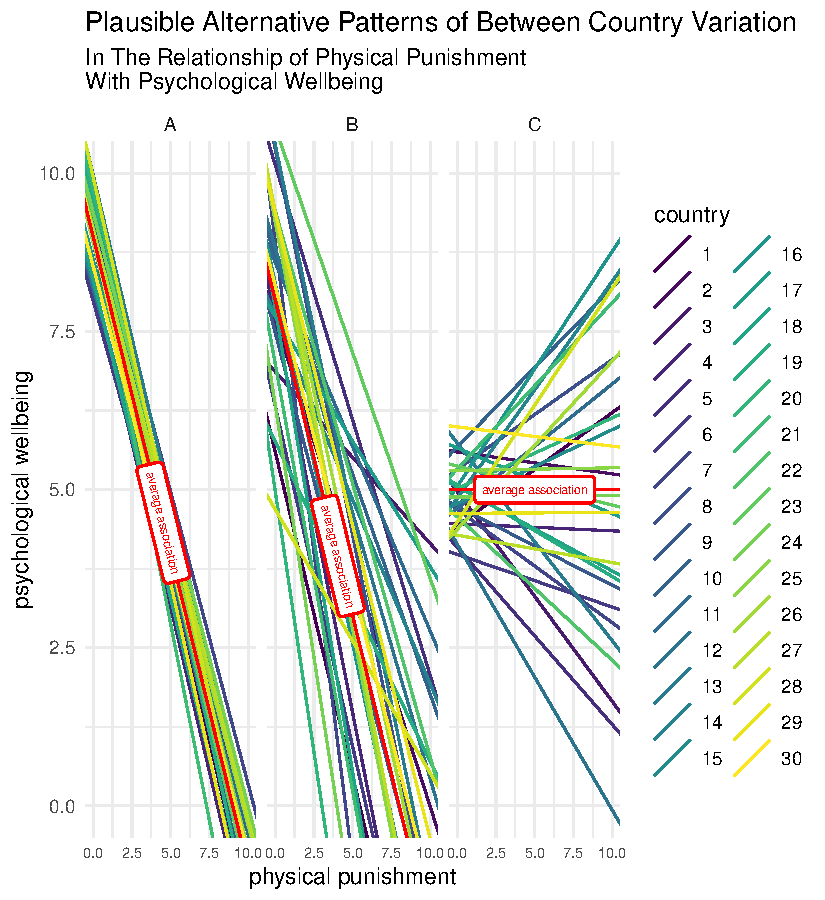
\includegraphics{./intro_files/figure-pdf/fig-variation1-1.pdf}

}

\caption{\label{fig-variation1}Plausible Alternative Patterns of Between
Country Variation}

\end{figure}

In Panel A, there is some variation in the \emph{intercept}, which is
equivalent to saying that there is some variation in the average level
of psychological well-being across countries. When we look at the slope
of the country-specific regression lines in Panel A, we notice that
there is little variation in these \emph{slopes}. Put another way, there
is a great amount of consistency in the slopes of the country-specific
regression lines: parental use of physical punishment is consistently
associated with decreases in child psychological wellbeing across
countries.

In Panel B, the situation is different. There is more variation in the
\emph{intercept}, that is, more variation between countries in the
initial or average amount of psychological well-being. There is also
more variation in the \emph{slopes} of the country-specific regression
lines. While the average association between physical punishment and
psychological well-being is very similar to that in Panel A, there is
more variation across countries, in the relationship of physical
punishment and child psychological wellbeing, which would likely merit
exploration were one considering developing programs, policies or
interventions for different countries.

Lastly, the pattern of variation in Panel C is considerably different
from either Panel A or Panel B. The average association of physical
punishment with psychological well-being in the hypothetical scenario
represented by Panel C is approximately 0. There is some variation in
the \emph{intercepts} of the country-specific regression lines.
Additionally, there is considerable variation in the \emph{slopes} of
the country-specific regression line, suggesting that the use of
physical punishment might be beneficial in some countries, and
detrimental in others.

Empirically, data generally suggest a scenario somewhere between Panel A
and Panel B, but these different hypothetical scenarios afford us the
opportunity to think about possible patterns of variation.

A second pedagogically helpful example might be obtained if we flip the
slopes in the diagram, and consider a different set of independent
variables, perhaps some kind of treatment or intervention designed to
improve psychological well-being.

\begin{Shaded}
\begin{Highlighting}[]
\FunctionTok{tribble}\NormalTok{(}
  \SpecialCharTok{\textasciitilde{}}\NormalTok{panel, }\SpecialCharTok{\textasciitilde{}}\NormalTok{beta0, }\SpecialCharTok{\textasciitilde{}}\NormalTok{beta1, }\SpecialCharTok{\textasciitilde{}}\NormalTok{u0, }\SpecialCharTok{\textasciitilde{}}\NormalTok{u1, }\SpecialCharTok{\textasciitilde{}}\NormalTok{label,}
  \StringTok{"A"}\NormalTok{, }\DecValTok{1}\NormalTok{, }\DecValTok{1}\NormalTok{, .}\DecValTok{5}\NormalTok{, .}\DecValTok{1}\NormalTok{, }\StringTok{"average association"}\NormalTok{,}
  \StringTok{"B"}\NormalTok{, }\DecValTok{1}\NormalTok{, }\DecValTok{1}\NormalTok{, }\FloatTok{1.5}\NormalTok{, .}\DecValTok{5}\NormalTok{, }\StringTok{"average association"}\NormalTok{,}
  \StringTok{"C"}\NormalTok{, }\DecValTok{5}\NormalTok{, }\DecValTok{0}\NormalTok{, .}\DecValTok{5}\NormalTok{, .}\DecValTok{25}\NormalTok{, }\StringTok{"average association"}\NormalTok{) }\SpecialCharTok{\%\textgreater{}\%} 
  \FunctionTok{uncount}\NormalTok{(}\AttributeTok{weights =} \DecValTok{30}\NormalTok{) }\SpecialCharTok{\%\textgreater{}\%}
  \FunctionTok{group\_by}\NormalTok{(panel) }\SpecialCharTok{\%\textgreater{}\%}
  \FunctionTok{mutate}\NormalTok{(}\AttributeTok{country =} \FunctionTok{factor}\NormalTok{(}\FunctionTok{row\_number}\NormalTok{())) }\SpecialCharTok{\%\textgreater{}\%}
  \FunctionTok{ungroup}\NormalTok{() }\SpecialCharTok{\%\textgreater{}\%}
  \FunctionTok{rowwise}\NormalTok{() }\SpecialCharTok{\%\textgreater{}\%}
  \FunctionTok{mutate}\NormalTok{(}\AttributeTok{intercept =}\NormalTok{ beta0 }\SpecialCharTok{+} \FunctionTok{rnorm}\NormalTok{(}\DecValTok{1}\NormalTok{, }\DecValTok{0}\NormalTok{, u0),}
         \AttributeTok{slope =}\NormalTok{ beta1 }\SpecialCharTok{+} \FunctionTok{rnorm}\NormalTok{(}\DecValTok{1}\NormalTok{, }\DecValTok{0}\NormalTok{, u1)) }\SpecialCharTok{\%\textgreater{}\%}
  \FunctionTok{ggplot}\NormalTok{() }\SpecialCharTok{+}
  \FunctionTok{geom\_abline}\NormalTok{(}\FunctionTok{aes}\NormalTok{(}\AttributeTok{intercept =}\NormalTok{ intercept, }
                  \AttributeTok{slope =}\NormalTok{ slope,}
                  \AttributeTok{color =}\NormalTok{ country)) }\SpecialCharTok{+}
  \FunctionTok{geom\_labelabline}\NormalTok{(}\FunctionTok{aes}\NormalTok{(}\AttributeTok{intercept =}\NormalTok{ beta0,}
                       \AttributeTok{slope =}\NormalTok{ beta1,}
                       \AttributeTok{label =}\NormalTok{ label),}
                   \AttributeTok{color =} \StringTok{"red"}\NormalTok{,}
                   \AttributeTok{size =} \DecValTok{2}\NormalTok{) }\SpecialCharTok{+}
  \FunctionTok{facet\_wrap}\NormalTok{(}\SpecialCharTok{\textasciitilde{}}\NormalTok{panel) }\SpecialCharTok{+}
  \FunctionTok{labs}\NormalTok{(}\AttributeTok{title =} \StringTok{"Considering an Intervention or Treatment Across Countries"}\NormalTok{,}
       \AttributeTok{x =} \StringTok{"hypothetical intervention"}\NormalTok{,}
       \AttributeTok{y =} \StringTok{"psychological wellbeing"}\NormalTok{) }\SpecialCharTok{+}
  \FunctionTok{xlim}\NormalTok{(}\DecValTok{0}\NormalTok{,}\DecValTok{10}\NormalTok{) }\SpecialCharTok{+}
  \FunctionTok{ylim}\NormalTok{(}\DecValTok{0}\NormalTok{,}\DecValTok{10}\NormalTok{) }\SpecialCharTok{+}
  \FunctionTok{scale\_color\_viridis\_d}\NormalTok{() }\SpecialCharTok{+}
  \FunctionTok{theme\_minimal}\NormalTok{() }\SpecialCharTok{+}
  \FunctionTok{theme}\NormalTok{(}\AttributeTok{axis.text.x =} \FunctionTok{element\_text}\NormalTok{(}\AttributeTok{size =} \FunctionTok{rel}\NormalTok{(.}\DecValTok{75}\NormalTok{)))}
\end{Highlighting}
\end{Shaded}

\begin{figure}[H]

{\centering 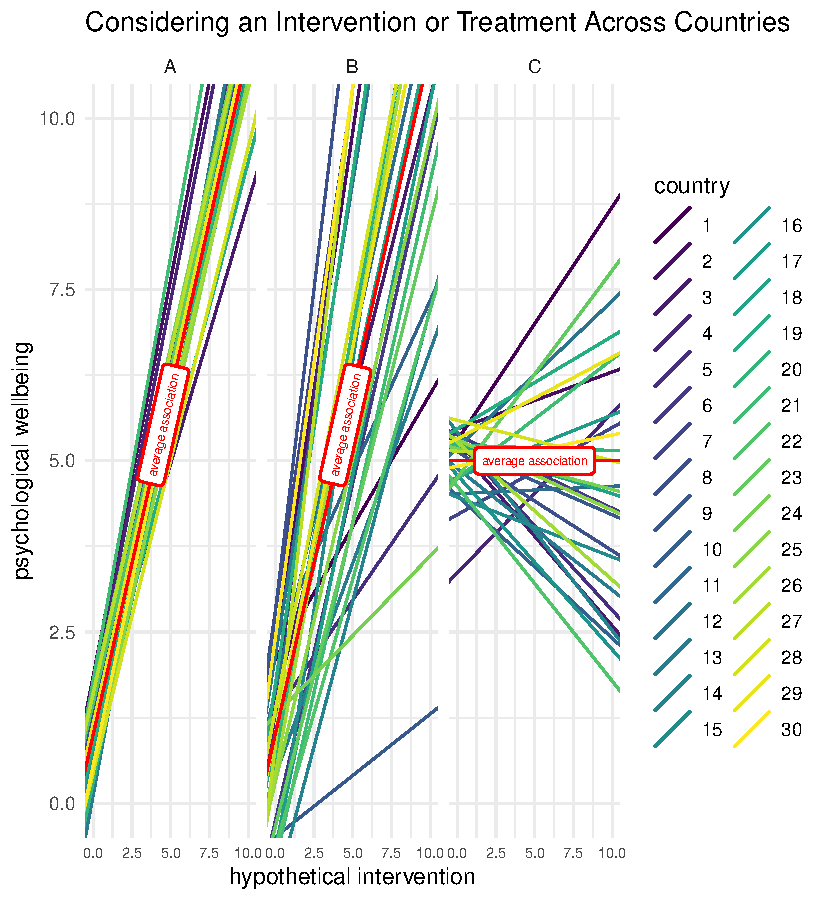
\includegraphics{./intro_files/figure-pdf/fig-variation2-1.pdf}

}

\caption{\label{fig-variation2}Considering an Intervention or Treatment
Across Countries}

\end{figure}

We see a similar pattern as before, but the use of a different
substantive example may be illustrative.

In Panel A, there is relative consistency in the initial levels of
psychological well-being across countries, as well as consistency in the
degree to which the intervention is associated with improvements in
psychological well-being across countries.

In Panel B, we see more variation in both initial levels of
psychological well-being, but also more variation in the association of
the intervention with improvements in psychological well-being.

Lastly, in Panel C, we note an overall association of the intervention
with psychological well-being that is close to zero. However
associations vary widely by countries. In some countries there appears
to be evidence that the intervention is beneficial, while in other
countries there appears to be evidence that the intervention is not
beneficial, or even possibly harmful.

Thus, I emphasize an approach to multilevel modeling that sees
multilevel modeling as the \emph{study of variation}, not simply
\emph{accounting for variation}, or \emph{controlling for variation}.

\begin{quote}
``\ldots universal theorizing requires adequately sampled (i.e.,
diverse) data and better appreciation of issues of comparability and the
most powerful theories ought to predict and explain variation, not sweep
variation under the rug.'' (Blasi et al., 2022)
\end{quote}

Again, sophisticated treatments of all of the ideas are available in one
form or another across the excellent textbooks on multilevel modeling
(Kreft \& de Leeuw, 1998; Luke, 2004; Rabe-Hesketh \& Skrondal, 2012;
Raudenbush \& Bryk, 2002; Singer \& Willett, 2003). However, some of
these ideas appear less often in applied research, and my intention here
is to make the application of these ideas to applied research more
clear.

\bookmarksetup{startatroot}

\hypertarget{simulated-multi-country-multilevel-data}{%
\chapter{Simulated Multi-Country (Multilevel)
Data}\label{simulated-multi-country-multilevel-data}}

\begin{Shaded}
\begin{Highlighting}[]
\FunctionTok{library}\NormalTok{(haven) }\CommentTok{\# read Stata}

\FunctionTok{library}\NormalTok{(dplyr) }\CommentTok{\# data wrangling}
\end{Highlighting}
\end{Shaded}

\begin{verbatim}

Attaching package: 'dplyr'
\end{verbatim}

\begin{verbatim}
The following objects are masked from 'package:stats':

    filter, lag
\end{verbatim}

\begin{verbatim}
The following objects are masked from 'package:base':

    intersect, setdiff, setequal, union
\end{verbatim}

\begin{Shaded}
\begin{Highlighting}[]
\FunctionTok{library}\NormalTok{(gt) }\CommentTok{\# beautiful tables}

\FunctionTok{library}\NormalTok{(ggplot2) }\CommentTok{\# beautiful graphs}

\FunctionTok{library}\NormalTok{(pander) }\CommentTok{\# tables for PDF}
\end{Highlighting}
\end{Shaded}

I use simulated data in this example. Data come from 30 hypothetical
countries. Data contain measures of a few key aspects of parenting that
have proven salient in the empirical literature on parenting to date:
parental \texttt{warmth}, and \texttt{physical\ punishment}. Both
parenting measures are normally distributed variables. Our
\texttt{outcome} is conceptualized as a positive mental health outcome
or behavioral outcome, and higher levels of \texttt{outcome} are
considered to be better. Statistically, the data are clustered within
countries.

In this simulation, I construct the data so that \texttt{warmth} is
positively related to the \texttt{outcome}, while
\texttt{physical\ punishment} is negatively related to the
\texttt{outcome}.

\begin{Shaded}
\begin{Highlighting}[]
\NormalTok{simulated\_multilevel\_data }\OtherTok{\textless{}{-}}
  \FunctionTok{read\_dta}\NormalTok{(}\StringTok{"./simulate{-}and{-}analyze{-}multilevel{-}data/simulated\_multilevel\_data.dta"}\NormalTok{)}

\NormalTok{simulated\_multilevel\_data }\OtherTok{\textless{}{-}}\NormalTok{ simulated\_multilevel\_data }\SpecialCharTok{\%\textgreater{}\%} 
  \FunctionTok{select}\NormalTok{(id, country,}
\NormalTok{         warmth,}
\NormalTok{         physical\_punishment,}
\NormalTok{         outcome)}
\end{Highlighting}
\end{Shaded}

\begin{Shaded}
\begin{Highlighting}[]
\NormalTok{pander}\SpecialCharTok{::}\FunctionTok{pander}\NormalTok{(}\FunctionTok{head}\NormalTok{(simulated\_multilevel\_data))}
\end{Highlighting}
\end{Shaded}

\hypertarget{tbl-simulateddata}{}
\begin{longtable}[]{@{}
  >{\centering\arraybackslash}p{(\columnwidth - 8\tabcolsep) * \real{0.0694}}
  >{\centering\arraybackslash}p{(\columnwidth - 8\tabcolsep) * \real{0.1389}}
  >{\centering\arraybackslash}p{(\columnwidth - 8\tabcolsep) * \real{0.1250}}
  >{\centering\arraybackslash}p{(\columnwidth - 8\tabcolsep) * \real{0.3056}}
  >{\centering\arraybackslash}p{(\columnwidth - 8\tabcolsep) * \real{0.1389}}@{}}
\caption{\label{tbl-simulateddata}Simulated Multilevel
Data}\tabularnewline
\toprule()
\begin{minipage}[b]{\linewidth}\centering
id
\end{minipage} & \begin{minipage}[b]{\linewidth}\centering
country
\end{minipage} & \begin{minipage}[b]{\linewidth}\centering
warmth
\end{minipage} & \begin{minipage}[b]{\linewidth}\centering
physical\_punishment
\end{minipage} & \begin{minipage}[b]{\linewidth}\centering
outcome
\end{minipage} \\
\midrule()
\endfirsthead
\toprule()
\begin{minipage}[b]{\linewidth}\centering
id
\end{minipage} & \begin{minipage}[b]{\linewidth}\centering
country
\end{minipage} & \begin{minipage}[b]{\linewidth}\centering
warmth
\end{minipage} & \begin{minipage}[b]{\linewidth}\centering
physical\_punishment
\end{minipage} & \begin{minipage}[b]{\linewidth}\centering
outcome
\end{minipage} \\
\midrule()
\endhead
1 & 15 & 129.6 & 84.86 & 685.3 \\
2 & 24 & 106.2 & 90.91 & 330.5 \\
3 & 11 & 83.41 & 95.94 & -130.8 \\
4 & 8 & 90.59 & 96 & 100.5 \\
5 & 21 & 95.06 & 85.3 & 149.1 \\
6 & 20 & 66.6 & 102.3 & 238.1 \\
\bottomrule()
\end{longtable}

\begin{Shaded}
\begin{Highlighting}[]
\FunctionTok{ggplot}\NormalTok{(simulated\_multilevel\_data,}
       \FunctionTok{aes}\NormalTok{(}\AttributeTok{x =}\NormalTok{ warmth,}
           \AttributeTok{y =}\NormalTok{ outcome,}
           \AttributeTok{color =} \FunctionTok{factor}\NormalTok{(country))) }\SpecialCharTok{+}
  \CommentTok{\# geom\_point() +}
  \FunctionTok{geom\_smooth}\NormalTok{(}\AttributeTok{method =} \StringTok{"lm"}\NormalTok{) }\SpecialCharTok{+}
  \FunctionTok{scale\_color\_viridis\_d}\NormalTok{(}\AttributeTok{name =} \StringTok{"country"}\NormalTok{) }\SpecialCharTok{+}
  \FunctionTok{labs}\NormalTok{(}\AttributeTok{title =} \StringTok{"Desirable Mental Health Outcome by Parental Warmth"}\NormalTok{,}
       \AttributeTok{subtitle =} \StringTok{"By Country"}\NormalTok{,}
       \AttributeTok{caption =} \StringTok{"Simulated Data"}\NormalTok{,}
       \AttributeTok{x =} \StringTok{"parental warmth"}\NormalTok{,}
       \AttributeTok{y =} \StringTok{"desirable mental health outcome"}\NormalTok{) }\SpecialCharTok{+}
  \FunctionTok{theme\_minimal}\NormalTok{() }
\end{Highlighting}
\end{Shaded}

\begin{verbatim}
`geom_smooth()` using formula = 'y ~ x'
\end{verbatim}

\begin{figure}[H]

{\centering 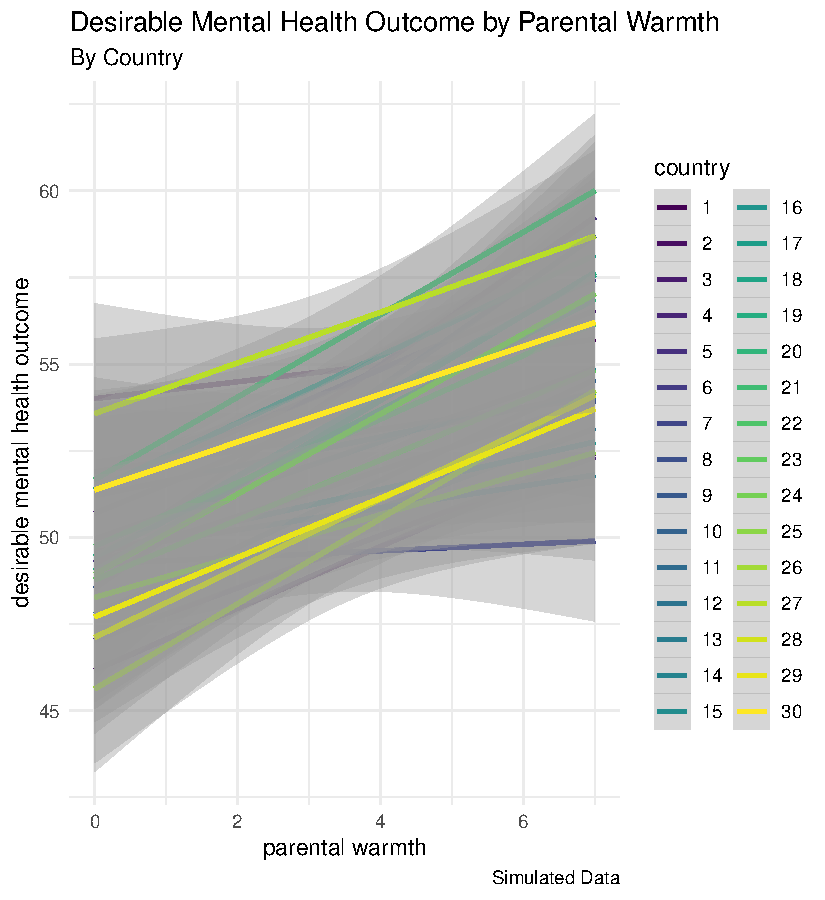
\includegraphics{./simulated-multi-country-data_files/figure-pdf/fig-data-1.pdf}

}

\caption{\label{fig-data}Graph of Simulated Data}

\end{figure}

\bookmarksetup{startatroot}

\hypertarget{sec-software}{%
\chapter{Software}\label{sec-software}}

In this document, I use Stata (StataCorp, 2021b) to analyze data. Stata
is my software of choice in this document because of Stata's overall
ease of use and intuitiveness. The creators of Stata have created a
powerful program that is extremely simple to use, but with a wide range
of both basic and advanced statistical capabilities.

The general idea of most Stata commands is:

\texttt{do\_something\ to\_a\_variable\_or\_variables,\ options}

Often it is not necessary to use any options since the authors of Stata
have done such a good job of thinking about the defaults.

For the sake of illustration, a few Stata commands are listed below.

\hypertarget{tbl-Statacommands}{}
\begin{longtable}[]{@{}ll@{}}
\caption{\label{tbl-Statacommands}Example Stata Commands}\tabularnewline
\toprule()
Task & Command \\
\midrule()
\endfirsthead
\toprule()
Task & Command \\
\midrule()
\endhead
Open data & \texttt{use\ mydata.dta} \\
Descriptive statistics & \texttt{summarize\ x\ y} \\
Frequencies & \texttt{tabulate\ x} \\
Correlation & \texttt{corr\ x\ y} \\
Regression & \texttt{regress\ y\ x} \\
Logistic Regression & \texttt{logit\ y\ x,\ or} \footnote{Here we use
  the \texttt{,or} option to ask for \emph{odds ratios} instead of
  \emph{logit coefficients}.} \\
Multilevel Model & \texttt{mixed\ y\ x\ \textbar{}\textbar{}\ group:} \\
\bottomrule()
\end{longtable}

It is this multilevel syntax,
\texttt{mixed\ y\ x\ \textbar{}\textbar{}\ group:} that we will be using
throughout this document.

\bookmarksetup{startatroot}

\hypertarget{conceptual-framework}{%
\chapter{Conceptual Framework}\label{conceptual-framework}}

\begin{Shaded}
\begin{Highlighting}[]
\FunctionTok{library}\NormalTok{(ggplot2) }\CommentTok{\# beautiful graphs}

\FunctionTok{library}\NormalTok{(geomtextpath) }\CommentTok{\# path geoms}

\FunctionTok{library}\NormalTok{(dplyr) }\CommentTok{\# data wrangling}
\end{Highlighting}
\end{Shaded}

\begin{verbatim}

Attaching package: 'dplyr'
\end{verbatim}

\begin{verbatim}
The following objects are masked from 'package:stats':

    filter, lag
\end{verbatim}

\begin{verbatim}
The following objects are masked from 'package:base':

    intersect, setdiff, setequal, union
\end{verbatim}

\begin{Shaded}
\begin{Highlighting}[]
\FunctionTok{library}\NormalTok{(tidyr) }\CommentTok{\# data tidying}

\FunctionTok{library}\NormalTok{(pander) }\CommentTok{\# nice tables}

\CommentTok{\# library(gt) \# beautiful tables}
\end{Highlighting}
\end{Shaded}

\hypertarget{units-of-analysis}{%
\section{Units of Analysis}\label{units-of-analysis}}

When confronted with multilevel data, one has a number of choices about
the units of analysis: one could consider individuals to be the units of
analysis; or, one could consider the larger social units to be the units
of analyses. With multilevel analytic methods, one is able to avoid this
false dichotomy, and to conceptualize the data from a multilevel
perspective, wherein both individuals and social units are different
levels of the same analysis. I discuss some of the statistical
considerations of different ideas about the units of analysis in
Section~\ref{sec-wrongapproaches}

\begin{Shaded}
\begin{Highlighting}[]
\NormalTok{DiagrammeR}\SpecialCharTok{::}\FunctionTok{grViz}\NormalTok{(}\StringTok{"}

\StringTok{digraph C \{}

\StringTok{rankdir=\textquotesingle{}LR\textquotesingle{}}

\StringTok{    subgraph cluster\_2 \{}
\StringTok{    }
\StringTok{    label = \textquotesingle{}Level 2: Social Units\textquotesingle{}}

\StringTok{  L2 }
\StringTok{  }
\StringTok{    \}}
\StringTok{    }
\StringTok{    subgraph cluster\_1 \{}
\StringTok{    }
\StringTok{    label = \textquotesingle{}Level 1: Individuals\textquotesingle{}}

\StringTok{  L1 {-}\textgreater{} y}
\StringTok{  L2 {-}\textgreater{} y}
\StringTok{    \}  }
\StringTok{    }

\StringTok{\}"}\NormalTok{)}
\end{Highlighting}
\end{Shaded}

\begin{figure}

{\centering 

}

\caption{\label{fig-conceptual}Conceptual Framework}

\end{figure}

\hypertarget{variables-and-processes-at-multiple-levels}{%
\section{Variables and Processes at Multiple
Levels}\label{variables-and-processes-at-multiple-levels}}

\begin{Shaded}
\begin{Highlighting}[]
\NormalTok{conceptuallevel }\OtherTok{\textless{}{-}} \FunctionTok{c}\NormalTok{(}\DecValTok{1}\NormalTok{,}\DecValTok{2}\NormalTok{,}\DecValTok{2}\NormalTok{)}
\NormalTok{statisticallevel1 }\OtherTok{\textless{}{-}} \FunctionTok{c}\NormalTok{(}\StringTok{"Individual response about parenting or mental health"}\NormalTok{,}
                       \StringTok{"Individual response about community"}\NormalTok{,}
                       \StringTok{"N/A"}\NormalTok{)}

\NormalTok{statisticallevel2 }\OtherTok{\textless{}{-}} \FunctionTok{c}\NormalTok{(}\StringTok{"Aggregated responses about parenting or mental health"}\NormalTok{,}
                       \StringTok{"Aggregated response about community"}\NormalTok{,}
                       \StringTok{"Administrative indicator of social unit"}\NormalTok{)}

\NormalTok{conceptualframework }\OtherTok{\textless{}{-}} \FunctionTok{data.frame}\NormalTok{(conceptuallevel,}
\NormalTok{                                  statisticallevel1,}
\NormalTok{                                  statisticallevel2)}

\NormalTok{pander}\SpecialCharTok{::}\FunctionTok{pander}\NormalTok{(conceptualframework)}
\end{Highlighting}
\end{Shaded}

\hypertarget{tbl-variablelevel}{}
\begin{longtable}[]{@{}
  >{\centering\arraybackslash}p{(\columnwidth - 4\tabcolsep) * \real{0.2338}}
  >{\centering\arraybackslash}p{(\columnwidth - 4\tabcolsep) * \real{0.3766}}
  >{\centering\arraybackslash}p{(\columnwidth - 4\tabcolsep) * \real{0.3896}}@{}}
\caption{\label{tbl-variablelevel}Multiple Levels of
Variables}\tabularnewline
\toprule()
\begin{minipage}[b]{\linewidth}\centering
conceptuallevel
\end{minipage} & \begin{minipage}[b]{\linewidth}\centering
statisticallevel1
\end{minipage} & \begin{minipage}[b]{\linewidth}\centering
statisticallevel2
\end{minipage} \\
\midrule()
\endfirsthead
\toprule()
\begin{minipage}[b]{\linewidth}\centering
conceptuallevel
\end{minipage} & \begin{minipage}[b]{\linewidth}\centering
statisticallevel1
\end{minipage} & \begin{minipage}[b]{\linewidth}\centering
statisticallevel2
\end{minipage} \\
\midrule()
\endhead
1 & Individual response about parenting or mental health & Aggregated
responses about parenting or mental health \\
2 & Individual response about community & Aggregated response about
community \\
2 & N/A & Administrative indicator of social unit \\
\bottomrule()
\end{longtable}

In this document, I distinguish between \emph{conceptual} and
\emph{statistical} levels.

By \emph{conceptual} level, I refer to whether a variable is
\emph{conceptualized} to be measure of an \emph{individual} level
characteristic, such as parenting or mental health, or a
\emph{community} level construct, such as community collective efficacy,
or community safety.

By \emph{statistical} level, I refer to whether a variable measures an
\emph{individual} response, or an \emph{aggregated} response.

\begin{itemize}
\item
  Thus, \(\text{mental health}_{ij}\) or \(\text{parenting}_{ij}\) would
  be considered in the terminology that I am using to be a variable both
  \emph{conceptually} and \emph{statistically} at Level 1.
\item
  \(\overline{\text{mental health}_{.j}}\) or
  \(\overline{\text{parenting}_{.j}}\) would be variables that
  \emph{conceptually} come from Level 1 responses, but are
  \emph{statistically} aggregated to Level 2.
\item
  Using my terminology, \(\text{community collective efficacy}_{ij}\) or
  \(\text{community safety}_{ij}\) would be considered to be a variable
  both \emph{conceptually} at Level 2, but \emph{statistically} at Level
  1.
\item
  \(\overline{\text{community collective efficacy}_{.j}}\) or
  \(\overline{\text{community safety}_{.j}}\) would be variables that
  \emph{conceptually} come from Level 2 responses, but are
  \emph{statistically} aggregated to Level 2.
\end{itemize}

Some variables only exist at Level 2, and their Level 1 counterparts are
undefined. For example, the size of a school, neighborhood, or country,
is inherently a Level 2 variable, with no Level 1 counterpart.
Similarly, some administrative indicators, such as the Gini level of
inequality, while developed by calculating across Level 1 responses,
have no easily definable Level 1 counterpart.

\bookmarksetup{startatroot}

\hypertarget{the-cross-sectional-multilevel-model}{%
\chapter{The Cross Sectional Multilevel
Model}\label{the-cross-sectional-multilevel-model}}

\begin{Shaded}
\begin{Highlighting}[]
\FunctionTok{library}\NormalTok{(haven) }\CommentTok{\# read Stata}

\FunctionTok{library}\NormalTok{(tibble) }\CommentTok{\# data frames}

\FunctionTok{library}\NormalTok{(ggplot2) }\CommentTok{\# beautiful graphs}

\FunctionTok{library}\NormalTok{(geomtextpath) }\CommentTok{\# path geoms}

\FunctionTok{library}\NormalTok{(dplyr) }\CommentTok{\# data wrangling}
\end{Highlighting}
\end{Shaded}

\begin{verbatim}

Attaching package: 'dplyr'
\end{verbatim}

\begin{verbatim}
The following objects are masked from 'package:stats':

    filter, lag
\end{verbatim}

\begin{verbatim}
The following objects are masked from 'package:base':

    intersect, setdiff, setequal, union
\end{verbatim}

\begin{Shaded}
\begin{Highlighting}[]
\FunctionTok{library}\NormalTok{(tidyr) }\CommentTok{\# data tidying}

\FunctionTok{library}\NormalTok{(pander) }\CommentTok{\# nice tables}

\CommentTok{\# library(gt) \# beautiful tables}
\end{Highlighting}
\end{Shaded}

\hypertarget{the-equation}{%
\section{The Equation}\label{the-equation}}

The equation for the multilevel model can be written in several ways: as
multiple levels of equations; or as a single equation. The advantage of
having multiple levels of equations is that these multiple equations
make clear the multiple levels of the data, and thus conform to an
initial understanding of how a multilevel model should be estimated.
However, results from multiple levels of equations quickly become
difficult to interpret, and thus, I will not spend a great deal of time
on discussing empirical results of the two level formulation. Whether
multiple levels of equations, or a single equation are employed, the
numerical results are the same.

\hypertarget{two-levels-of-equations}{%
\subsection{Two Levels of Equations}\label{two-levels-of-equations}}

I start with two levels of equations: Level 1 at the level of the
individual; and Level 2 at the level of the country.

\hypertarget{level-1-individuals}{%
\subsubsection{Level 1 (Individuals)}\label{level-1-individuals}}

\begin{equation}\protect\hypertarget{eq-MLM1}{}{y_{ij} = \beta_{0j} + \beta_{1j} x_{ij} + \beta_{2j} z_{ij} + \beta_{3j} t_{ij} + e_{ij}}\label{eq-MLM1}\end{equation}

\hypertarget{level-2-countries}{%
\subsubsection{Level 2 (Countries)}\label{level-2-countries}}

\begin{equation}\protect\hypertarget{eq-MLM2}{}{\beta_{0j} = \gamma_{00} + u_{0j}}\label{eq-MLM2}\end{equation}

\[\beta_{1j} = \gamma_{10} + u_{1j}\]

\[\beta_{2j} = \gamma_{20}\]

\[\beta_{3j} = \gamma_{30}\]

Here \(y_{ij}\) is the dependent variable, or outcome for the model. We
note that the \(ij\) subscripts indicate that this is outcome \(y\) for
individual \(i\) in country \(j\). Note that the outcome is at Level 1,
or the level of individuals. \(\beta_{0j}\) is a regression intercept,
and the other \(\beta\)'s\footnote{Technically, all of these \(\beta\)'s
  could be written as \(\beta_j\) since the multilevel model could be
  said to estimate a regression parameter for each group, in this case
  each country. One could even write \(\beta_{jk}\) to represent the
  regression parameter for the \(k^{th}\) independent variable the for
  the \(j^{th}\) group or country. To keep matters simple, I simply
  write \(\beta\) in most cases.} are regression slope parameters.
\(x_{ij}\) and \(z_{ij}\) are independent variables and \(t_{ij}\) is an
independent variable indicating the time at which different data points
are measured. I note that in this discussion I am \emph{not} considering
a model in which there are repeated observations on the same
individuals, although the multilevel model is certainly extensible to
such cases. \(u_{0j}\) is a random intercept for the \(\beta_{0j}\)
term, and \(u_{1j}\) is a random slope for the \(\beta_{1j}\) term,
indicating that we are modeling cross country variation in these
parameters. The other \(\beta\) terms are not modeled as having random
country level variation, although this could certainly be a possibility
in subsequent models.

In this formulation of the multilevel model, each regression parameter
\(\beta\) in the level 1 equation is the outcome of an equation at Level
2.

\hypertarget{one-level-of-equations}{%
\subsection{One Level of Equations}\label{one-level-of-equations}}

By simply substituting the values of the Level 2 equations into the
Level 1 equations, we obtain:

\begin{equation}\protect\hypertarget{eq-MLM}{}{y_{ij} = \beta_0 + \beta_1 x_{ij} + \beta_2 z_{ij} + \beta_3 t_{ij} + u_{0j} + u_{1j} \times x + e_{ij}}\label{eq-MLM}\end{equation}

Here again \(y_{ij}\) is the dependent variable, or outcome for the
model. \(\beta_0\) is a regression intercept, and the \(\beta\)'s are
regression parameters. \(x_{ij}\) and \(z_{ij}\) are independent
variables and \(t\) is an independent variable indicating the time at
which different data points.

While I purposely strive to keep the discussion of multilevel modeling
ideas somewhat general in this document, I generally think of \(y_{ij}\)
as a desirable or ``good'' outcome. \(x\) is often conceptualized as a
protective factor, while \(z\) is often conceptualized as a risk factor.

Thus, phrased less abstractly, and more concretely in terms of the ideas
of this document:

\begin{equation}\protect\hypertarget{eq-MLMsubstantive}{}{\text{outcome}_{ij} = \beta_0 + \beta_1 \text{parental warmth}_{ij} + \beta_2 \text{physical punishment}_{ij} + \beta_3 \text{time}_{ij} \ + }\label{eq-MLMsubstantive}\end{equation}

\[u_{0j} + u_{1j} \times \text{parental warmth} + e_{ij}\]

Drawing upon ideas from Chapter~\ref{sec-software}, this single level
equation can be easily represented in Stata syntax.

\texttt{mixed\ outcome\ warmth\ physical\_punishment\ \textbar{}\textbar{}\ country:\ warmth}

\hypertarget{sec-pvalues}{%
\section{Estimating Standard Errors And p Values}\label{sec-pvalues}}

\hypertarget{introduction-1}{%
\subsection{Introduction}\label{introduction-1}}

If the data are grouped, nested, or clustered, then this aspect of the
structure of the data needs to be accounted for. Bland \& Altman (1994)
describe a simulation in which grouped data are artificially generated
according to the following procedure.

\begin{quote}
``The data were generated from random numbers, and there is no relation
between X and Y at all. Firstly, values of X and Y were generated for
each `subject,' then a further random number was added to make the
individual observation.'' (Bland \& Altman, 1994)
\end{quote}

\begin{Shaded}
\begin{Highlighting}[]
\NormalTok{simulated\_clustered\_data }\OtherTok{\textless{}{-}}
  \FunctionTok{read\_dta}\NormalTok{(}\StringTok{"./simulate{-}and{-}analyze{-}multilevel{-}data/simulated\_clustered\_data.dta"}\NormalTok{)}
\end{Highlighting}
\end{Shaded}

The graph below illustrates the process of simulating the data.

\begin{Shaded}
\begin{Highlighting}[]
\FunctionTok{ggplot}\NormalTok{(simulated\_clustered\_data,}
       \FunctionTok{aes}\NormalTok{(}\AttributeTok{color =} \FunctionTok{factor}\NormalTok{(group\_numA),}
           \AttributeTok{label =}\NormalTok{ group\_numA)) }\SpecialCharTok{+}
  \FunctionTok{geom\_segment}\NormalTok{(}\FunctionTok{aes}\NormalTok{(}\AttributeTok{x =}\NormalTok{ x\_individualA, }
                \AttributeTok{y =}\NormalTok{ y\_individualA,}
                \AttributeTok{xend =}\NormalTok{ x\_groupA,}
                \AttributeTok{yend =}\NormalTok{ y\_groupA),}
               \AttributeTok{show.legend =} \ConstantTok{FALSE}\NormalTok{) }\SpecialCharTok{+}
  \FunctionTok{geom\_point}\NormalTok{(}\FunctionTok{aes}\NormalTok{(}\AttributeTok{x =}\NormalTok{ x\_groupA, }
                 \AttributeTok{y =}\NormalTok{ y\_groupA),}
             \AttributeTok{size =} \DecValTok{10}\NormalTok{,}
             \AttributeTok{alpha =} \DecValTok{1}\NormalTok{,}
             \AttributeTok{show.legend =} \ConstantTok{TRUE}\NormalTok{) }\SpecialCharTok{+} 
  \FunctionTok{geom\_text}\NormalTok{(}\FunctionTok{aes}\NormalTok{(}\AttributeTok{x =}\NormalTok{ x\_groupA,}
                \AttributeTok{y =}\NormalTok{ y\_groupA),}
            \AttributeTok{color =} \StringTok{"white"}\NormalTok{,}
            \AttributeTok{show.legend =} \ConstantTok{FALSE}\NormalTok{) }\SpecialCharTok{+}
  \FunctionTok{geom\_label}\NormalTok{(}\FunctionTok{aes}\NormalTok{(}\AttributeTok{x =}\NormalTok{ x\_individualA, }
                \AttributeTok{y =}\NormalTok{ y\_individualA),}
             \AttributeTok{show.legend =} \ConstantTok{FALSE}\NormalTok{,}
             \AttributeTok{size =} \DecValTok{3}\NormalTok{) }\SpecialCharTok{+} 
  \FunctionTok{labs}\NormalTok{(}\AttributeTok{title =} \StringTok{"Illustrating the Process of Simulating the Data"}\NormalTok{,}
       \AttributeTok{x =} \StringTok{"x"}\NormalTok{,}
       \AttributeTok{y =} \StringTok{"y"}\NormalTok{) }\SpecialCharTok{+}
  \FunctionTok{theme\_minimal}\NormalTok{() }\SpecialCharTok{+}
  \FunctionTok{scale\_color\_viridis\_d}\NormalTok{(}\AttributeTok{name =} \StringTok{"group"}\NormalTok{)}
\end{Highlighting}
\end{Shaded}

\begin{figure}[H]

{\centering 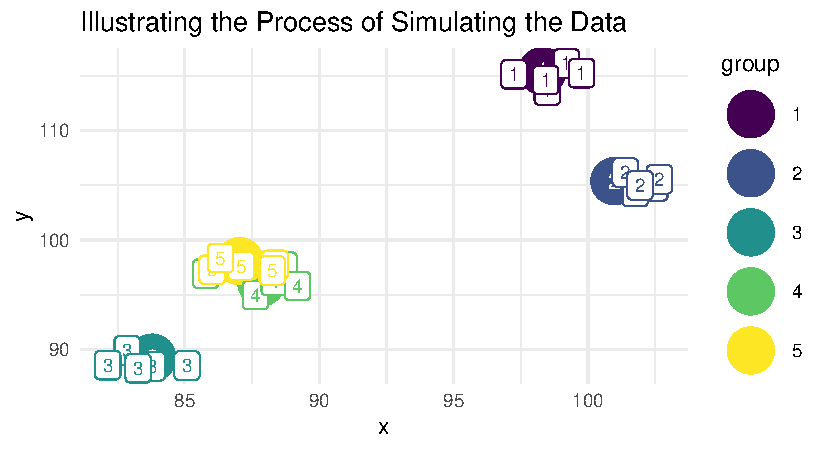
\includegraphics{./cross-sectional_files/figure-pdf/unnamed-chunk-3-1.pdf}

}

\caption{Simulated Clustered Data}

\end{figure}

\hypertarget{compare-ols-and-mlm}{%
\subsection{Compare OLS and MLM}\label{compare-ols-and-mlm}}

An analysis that is not aware of the grouped nature of the data will
give biased results, will mis-estimate standard errors, and importantly,
will often attribute statistical significance to some of the independent
variables when this is not appropriate (Bland \& Altman, 1994;
Raudenbush \& Bryk, 2002).

In the example below, we compare a simple ordinary least squares
analysis of the data with a multilevel model that accounts for the
clustered nature of the data.

The Stata syntax that we use for each analysis is:

\begin{itemize}
\tightlist
\item
  \texttt{regress\ y\ x}
\item
  \texttt{mixed\ y\ x\ \textbar{}\textbar{}\ group:}
\end{itemize}

\begin{longtable}[]{@{}lllll@{}}
\toprule()
& OLS & & MLM & \\
\midrule()
\endhead
x & 1.046 & ** & 0.039 & \\
Intercept & 4.488 & & 97.005 & ** \\
var(\_cons) & & & 74.523 & \\
var(e) & & & 0.594 & \\
Number of observations & 25 & & & \\
\bottomrule()
\end{longtable}

** p\textless.01, * p\textless.05

We see that in the ordinary least squares analysis, the independent
variable is judged to have a statistically significant association with
the dependent variable. The more appropriate multilevel model finds that
in fact the independent variable \(x\) is \emph{not} associated with
\(y\). Thus, the multilevel model provides more accurate results than
OLS in the presence of clustered data.

\hypertarget{sec-multilevelstructure}{%
\section{Multilevel Structure}\label{sec-multilevelstructure}}

Associations between two variables can be \emph{very different} (or even
\emph{reversed}) depending upon whether or not the analysis is ``aware''
of the grouped, nested, or clustered nature of the data (Gelman et al.,
2007). In the example presented here, the groups are countries, but
could as easily be neighborhoods, communities, or schools.

For pedagogical purposes, I use an example with very few clusters,
although it would be more appropriate to apply multilevel analysis to an
example with many more clusters e.g.~(\(N_\text{clusters} >= 30\))

A model that is ``aware'' of the clustered nature of the data may
provide very different--likely better--substantive conclusions than a
model that is not aware of the clustered nature of the data.

\hypertarget{use-some-data-simulated-for-this-particular-example}{%
\subsection{Use Some Data Simulated For This Particular
Example}\label{use-some-data-simulated-for-this-particular-example}}

\begin{Shaded}
\begin{Highlighting}[]
\NormalTok{multilevelstructure }\OtherTok{\textless{}{-}}
  \FunctionTok{read\_dta}\NormalTok{(}\StringTok{"./simulate{-}and{-}analyze{-}multilevel{-}data/multilevelstructure.dta"}\NormalTok{)}

\NormalTok{multilevelstructure}\SpecialCharTok{$}\NormalTok{country }\OtherTok{\textless{}{-}} \FunctionTok{factor}\NormalTok{(multilevelstructure}\SpecialCharTok{$}\NormalTok{country)}
\end{Highlighting}
\end{Shaded}

\hypertarget{graphs}{%
\subsection{Graphs}\label{graphs}}

\hypertarget{a-naive-graph}{%
\subsubsection{A ``Naive'' Graph}\label{a-naive-graph}}

This ``naive'' graph is unaware of the grouped nature of the data.
Notice that the overall regression line slopes downward, even though
there is some suggestion that \emph{within each group} the regression
lines may slope upward.

\begin{Shaded}
\begin{Highlighting}[]
\NormalTok{p0 }\OtherTok{\textless{}{-}} \FunctionTok{ggplot}\NormalTok{(multilevelstructure, }
             \FunctionTok{aes}\NormalTok{(}\AttributeTok{x =}\NormalTok{ x,}
                 \AttributeTok{y =}\NormalTok{ y)) }\SpecialCharTok{+}
  \FunctionTok{geom\_smooth}\NormalTok{(}\AttributeTok{method =} \StringTok{"lm"}\NormalTok{) }\SpecialCharTok{+}
  \FunctionTok{geom\_point}\NormalTok{() }\SpecialCharTok{+}
  \FunctionTok{labs}\NormalTok{(}\AttributeTok{title =} \StringTok{"y as a function of x"}\NormalTok{) }\SpecialCharTok{+}
  \FunctionTok{theme\_minimal}\NormalTok{()}

\NormalTok{p0  }\CommentTok{\# replay }
\end{Highlighting}
\end{Shaded}

\begin{verbatim}
`geom_smooth()` using formula = 'y ~ x'
\end{verbatim}

\begin{figure}[H]

{\centering 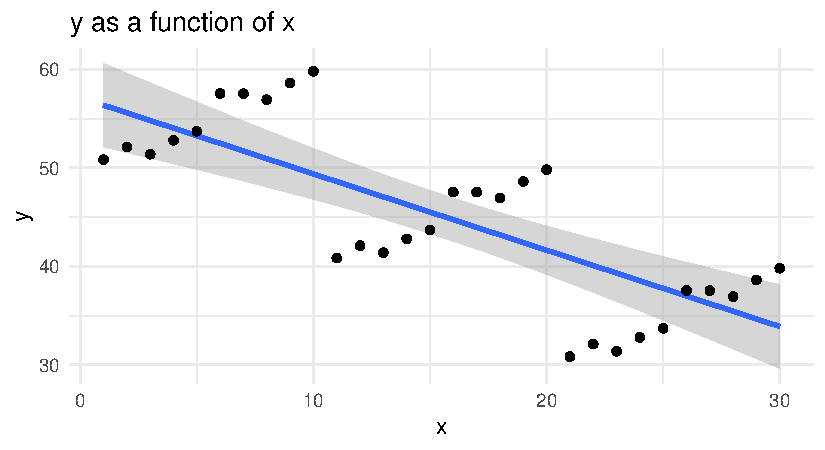
\includegraphics{./cross-sectional_files/figure-pdf/fig-naive-1.pdf}

}

\caption{\label{fig-naive}A `Naive' Graph}

\end{figure}

\hypertarget{an-aware-graph}{%
\subsubsection{An ``Aware'' Graph}\label{an-aware-graph}}

This ``aware'' graph is aware of the grouped nature of the data. The
graph is ``aware'' of the grouped or clustered nature of the data, and
provides indication that the regression lines \emph{when accounting for
group} slope upward.

\begin{Shaded}
\begin{Highlighting}[]
\FunctionTok{ggplot}\NormalTok{(multilevelstructure, }
             \FunctionTok{aes}\NormalTok{(}\AttributeTok{x =}\NormalTok{ x,}
                 \AttributeTok{y =}\NormalTok{ y,}
                 \AttributeTok{color =}\NormalTok{ country)) }\SpecialCharTok{+} \CommentTok{\# color is country}
  \FunctionTok{geom\_point}\NormalTok{() }\SpecialCharTok{+} 
  \FunctionTok{geom\_smooth}\NormalTok{(}\AttributeTok{method =} \StringTok{"lm"}\NormalTok{) }\SpecialCharTok{+} 
  \FunctionTok{scale\_color\_viridis\_d}\NormalTok{() }\SpecialCharTok{+}
  \FunctionTok{theme\_minimal}\NormalTok{()}
\end{Highlighting}
\end{Shaded}

\begin{verbatim}
`geom_smooth()` using formula = 'y ~ x'
\end{verbatim}

\begin{figure}[H]

{\centering 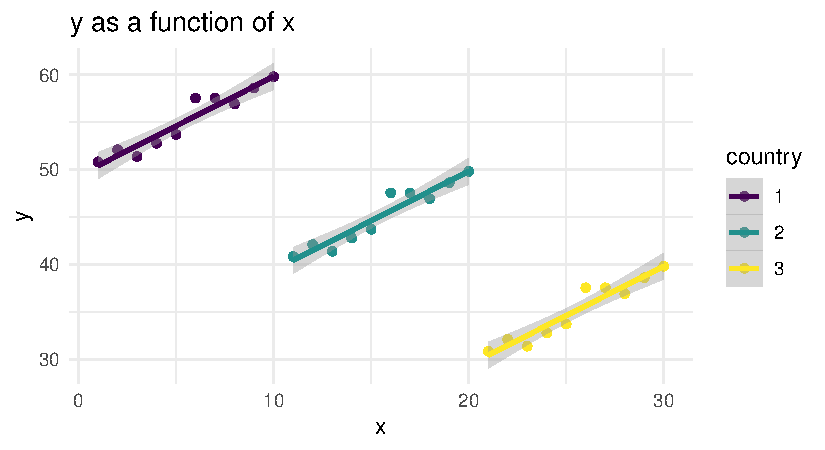
\includegraphics{./cross-sectional_files/figure-pdf/fig-aware-1.pdf}

}

\caption{\label{fig-aware}An `Aware' Graph}

\end{figure}

\hypertarget{regressions}{%
\subsection{Regressions}\label{regressions}}

\hypertarget{a-naive-ols-analysis-vs.-an-aware-mlm-analysis}{%
\subsubsection{A ``Naive'' OLS Analysis vs.~An ``Aware'' MLM
Analysis}\label{a-naive-ols-analysis-vs.-an-aware-mlm-analysis}}

The Stata syntax that we use for these analyses is:

\begin{itemize}
\tightlist
\item
  \texttt{regress\ y\ x}
\item
  \texttt{mixed\ y\ x\ \textbar{}\textbar{}\ country:}
\end{itemize}

The OLS model with only \emph{x} as a covariate is not aware of the
grouped structure of the data, and the coefficient for \emph{x} in the
OLS model reflects this. The coefficient for \emph{x} in the OLS model
is \emph{negative}, and statistically significant.

The multilevel model is aware of the grouped structure of the data, and
the coefficient for \emph{x} in the multilevel model reflects this. The
coefficient for \emph{x} in the multilevel model is \emph{positive}, and
statistically significant.

\begin{longtable}[]{@{}lllll@{}}
\toprule()
& OLS & & MLM & \\
\midrule()
\endhead
x & -0.771 & ** & 1.072 & ** \\
Intercept & 57.122 & ** & 28.553 & ** \\
var(\_cons) & & & 286.088 & \\
var(e) & & & 0.758 & \\
Number of observations & 30 & & & \\
\bottomrule()
\end{longtable}

** p\textless.01, * p\textless.05

\hypertarget{a-thought-experiment}{%
\subsection{A Thought Experiment}\label{a-thought-experiment}}

When might a situation like this arise in practice? This is surprisingly
difficult to think through.

Imagine that \emph{x} is a protective factor, or an intervention or
treatment. Imagine that \emph{y} is a desirable outcome, like improved
mental health or psychological well being.

Now imagine that residents of countries provide more of the protective
factor or more of the intervention in situations where there are lower
levels of the desirable outcome. If one thinks about it, this is a very
plausible situation.

\begin{quote}
A naive analysis that was unaware of the grouped nature of the data
would therefore misconstrue the results, suggesting that the
intervention was harmful, when it was in fact helpful.
\end{quote}

\begin{Shaded}
\begin{Highlighting}[]
\NormalTok{p0 }\SpecialCharTok{+} 
  \FunctionTok{geom\_point}\NormalTok{(}\FunctionTok{aes}\NormalTok{(}\AttributeTok{color =}\NormalTok{ country)) }\SpecialCharTok{+} \CommentTok{\# points with country color}
  \FunctionTok{geom\_smooth}\NormalTok{(}\FunctionTok{aes}\NormalTok{(}\AttributeTok{color =}\NormalTok{ country), }\CommentTok{\# smoothers with country color}
              \AttributeTok{method =} \StringTok{"lm"}\NormalTok{) }\SpecialCharTok{+} 
  \FunctionTok{labs}\NormalTok{(}\AttributeTok{title =} \StringTok{"Desirable Outcome as a Function of Intervention or Treatment"}\NormalTok{,}
       \AttributeTok{x =} \StringTok{"intervention or treatment"}\NormalTok{,}
       \AttributeTok{y =} \StringTok{"desirable outcome"}\NormalTok{) }\SpecialCharTok{+}
  \FunctionTok{scale\_color\_viridis\_d}\NormalTok{()}
\end{Highlighting}
\end{Shaded}

\begin{verbatim}
`geom_smooth()` using formula = 'y ~ x'
`geom_smooth()` using formula = 'y ~ x'
\end{verbatim}

\begin{figure}[H]

{\centering 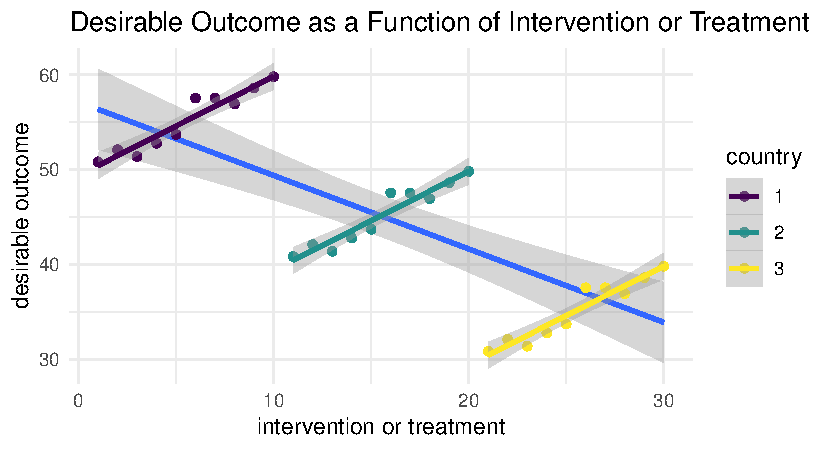
\includegraphics{./cross-sectional_files/figure-pdf/unnamed-chunk-9-1.pdf}

}

\caption{A Heuristic Example}

\end{figure}

These data are constructed to provide this kind of extreme example, but
it easy to see how multilevel thinking, and multilevel analysis may
provide better answers than one would get if one ignored the grouped
nature of the data.

\hypertarget{sec-regression}{%
\section{Regression With Simulated Multi-Country
Data}\label{sec-regression}}

Let's examine the results of a multilevel regression with the simulated
multicountry data. I will again imagine that the desirable outcome is an
outcome such as improved psychological wellbeing.

The Stata syntax that we use is:

\texttt{mixed\ outcome\ warmth\ physical\_punishment\ \textbar{}\textbar{}\ country:\ warmth}

\begin{longtable}[]{@{}lll@{}}
\toprule()
& cross\_sectional & \\
\midrule()
\endhead
warmth & 4.855 & ** \\
physical\_punishment & -3.242 & ** \\
Intercept & 30.930 & \\
var(warmth) & 0.800 & \\
var(\_cons) & 1018.485 & \\
var(e) & 2574.967 & \\
\bottomrule()
\end{longtable}

** p\textless.01, * p\textless.05

The data suggest that parental warmth is positively associated with the
desirable outcome, and that this result is statistically significant.
Parental use of physical punishment is associated with statistically
significant decreases in the desirable outcome. I note that there is
some variation in the \emph{constant} indicating that there is some
variation in the initial or average levels of the desirable
outcome--again improved psychological well-being--that is attributable
to country.

There is also some variation in the slope associated with parental
warmth that is attributable to country. Thus, while largely consistent,
the relationship of parental warmth with child outcomes differs somewhat
from country to country.

\hypertarget{summary-of-advantages-of-the-multilevel-model}{%
\section{Summary of Advantages Of The Multilevel
Model}\label{summary-of-advantages-of-the-multilevel-model}}

The discussion so far gives an idea of the advantages of the multilevel
model for studying intrinsically multilevel data: children in classrooms
or schools; individuals or families in neighborhoods; individuals or
families in countries. These advantages can be summarized below:

\begin{enumerate}
\def\labelenumi{\arabic{enumi}.}
\tightlist
\item
  Standard errors are estimated correctly as is statistical
  significance. This means that p values are correctly estimated
  accounting for the clustered or nested nature of the data. More
  colloquially, this most often means that we do not make the mistake of
  attributing statistical significance to a given risk or protective
  factor, when such a statistical significance is not warranted. Put
  even more straightforwardly correct estimation of standard errors and
  statistical significance prevents us from seeing results that are
  simply not present in the data, whether those concern risk factors or
  protective factors.
\item
  Regression coefficients are estimated correctly accounting for the
  clustered or nested structure of the data. If one does not account for
  the clustered or nested structure of the data, regression slopes can
  be estimated as negative when they are more correctly estimated as
  positive, or as null, or conversely estimated as positive when there
  are more correctly seen as negative (or null). Again, to phrase things
  in a more colloquial fashion, this means that we do not judge
  something to be a risk factor when it is in fact a protective factor
  or a null effect; or a protective factor when it is in fact a risk
  factor, or a null effect.\\
\item
  An increasing focus of statistical estimation is not to focus on
  particular regression parameters, but instead to predict outcomes for
  particular combinations of independent variables. Predictions from a
  multilevel model could be said to be best predictions in that groups
  are weighted by their precision, contributing to an estimate which
  makes better predictions than would a simple average. More
  colloquially, multilevel models allow us to predict outcomes better
  and more accurately than would be possible with simple or more naïve
  models.
\end{enumerate}

\hypertarget{predicted-values}{%
\section{Predicted Values}\label{predicted-values}}

According to \textbf{``Stein's Paradox''}, predictions from a multilevel
model may be better than the mean.

\textbf{shrinkage}

\hypertarget{variation}{%
\section{Variation}\label{variation}}

Above, in Section~\ref{sec-studyvariation}, I have referred to
multilevel models as the study of variation. Now that I have provided
some discussion of the multilevel model, more statistical ``unpacking''
of ideas about variation is warranted.

I provide again, for pedagogical purposes, the example substantive
equation that I have been using in this document.

\begin{equation}\protect\hypertarget{eq-MLMsubstantive2}{}{\text{outcome}_{ij} = \beta_0 + \beta_1 \text{parental warmth}_{ij} + \beta_2 \text{physical punishment}_{ij} + \beta_3 \text{time}_{ij} \ + }\label{eq-MLMsubstantive2}\end{equation}

\[u_{0j} + u_{1j} \times \text{parental warmth} + e_{ij}\]

\hypertarget{measured-and-unmeasured-variation}{%
\subsection{Measured and Unmeasured
Variation}\label{measured-and-unmeasured-variation}}

The first thing to note about the equation is that it can be divided
into measured and unmeasured variation.

This is most easily seen if we introduce the idea of an unconditional
model.

\hypertarget{unconditional-model}{%
\subsection{Unconditional Model}\label{unconditional-model}}

The unconditional model is a model with no \(x\)'s or covariates.

\begin{equation}\protect\hypertarget{eq-unconditional}{}{\text{outcome}_{ij} = \beta_0 + u_{0j} + e_{ij}}\label{eq-unconditional}\end{equation}

Here, \(\text{outcome}_{ij}\) is a function of an intercept \(\beta_0\),
a country specific error term, \(u_{0j}\), and an individual level error
term \(e_{ij}\).

Thus, all of the variation in \(\text{outcome}_{ij}\) is--given the
unconditional nature of our model--due to unmeasured variation at the
country and individual level.

\hypertarget{intra-class-correlation-coefficient}{%
\subsection{Intra-Class Correlation
Coefficient}\label{intra-class-correlation-coefficient}}

We then introduce a measure known as the Intra-Class Correlation
Coefficient, (ICC) that can be computed from this unconditional model.

\begin{equation}\protect\hypertarget{eq-ICC}{}{\text{ICC} = \frac{var(u_{0j})}{var(u_{0j}) + var(e_{ij})}}\label{eq-ICC}\end{equation}

Heuristically:

\begin{equation}\protect\hypertarget{eq-ICCheuristic}{}{\text{ICC} = \frac{\text{group level variation}}{\text{group level variation} + \text{individual level variation}}}\label{eq-ICCheuristic}\end{equation}

The ICC from the \emph{unconditional} model
(Equation~\ref{eq-unconditional}) is the most informative ICC as it
represents the amount of variation in the dependent variable that could
\emph{potentially} be explained by the grouping variable.

As we add covariates, \(x\)'s, to the model the ICC will most often
decrease.

\begin{Shaded}
\begin{Highlighting}[]
\FunctionTok{tribble}\NormalTok{(}
  \SpecialCharTok{\textasciitilde{}}\NormalTok{beta0, }\SpecialCharTok{\textasciitilde{}}\NormalTok{beta1, }\SpecialCharTok{\textasciitilde{}}\NormalTok{u0, }\SpecialCharTok{\textasciitilde{}}\NormalTok{u1,}
  \DecValTok{5}\NormalTok{, }\DecValTok{0}\NormalTok{, .}\DecValTok{5}\NormalTok{, .}\DecValTok{25}\NormalTok{) }\SpecialCharTok{\%\textgreater{}\%} 
  \FunctionTok{uncount}\NormalTok{(}\AttributeTok{weights =} \DecValTok{30}\NormalTok{) }\SpecialCharTok{\%\textgreater{}\%}
  \FunctionTok{mutate}\NormalTok{(}\AttributeTok{country =} \FunctionTok{factor}\NormalTok{(}\FunctionTok{row\_number}\NormalTok{())) }\SpecialCharTok{\%\textgreater{}\%}
  \FunctionTok{ungroup}\NormalTok{() }\SpecialCharTok{\%\textgreater{}\%}
  \FunctionTok{rowwise}\NormalTok{() }\SpecialCharTok{\%\textgreater{}\%}
  \FunctionTok{mutate}\NormalTok{(}\AttributeTok{intercept =}\NormalTok{ beta0 }\SpecialCharTok{+} \FunctionTok{rnorm}\NormalTok{(}\DecValTok{1}\NormalTok{, }\DecValTok{0}\NormalTok{, u0),}
         \AttributeTok{slope =}\NormalTok{ beta1 }\SpecialCharTok{+} \FunctionTok{rnorm}\NormalTok{(}\DecValTok{1}\NormalTok{, }\DecValTok{0}\NormalTok{, u1)) }\SpecialCharTok{\%\textgreater{}\%}
  \FunctionTok{ggplot}\NormalTok{() }\SpecialCharTok{+}
  \FunctionTok{geom\_abline}\NormalTok{(}\FunctionTok{aes}\NormalTok{(}\AttributeTok{intercept =}\NormalTok{ intercept, }
                  \AttributeTok{slope =}\NormalTok{ slope),}
              \AttributeTok{color =} \StringTok{"grey"}\NormalTok{) }\SpecialCharTok{+}
  \FunctionTok{annotate}\NormalTok{(}\AttributeTok{geom =} \StringTok{"point"}\NormalTok{, }
           \AttributeTok{x =} \DecValTok{0}\NormalTok{, }
           \AttributeTok{y =} \DecValTok{5}\NormalTok{, }
           \AttributeTok{color =} \StringTok{"orange"}\NormalTok{,}
           \AttributeTok{alpha =}\NormalTok{ .}\DecValTok{5}\NormalTok{,}
           \AttributeTok{size =} \DecValTok{17}\NormalTok{) }\SpecialCharTok{+}
  \FunctionTok{annotate}\NormalTok{(}\StringTok{"text"}\NormalTok{, }
           \AttributeTok{x =} \FloatTok{1.5}\NormalTok{, }
           \AttributeTok{y =} \FloatTok{2.5}\NormalTok{, }
           \AttributeTok{label =} \StringTok{"variation in y"}\NormalTok{,}
           \AttributeTok{color =} \StringTok{"red"}\NormalTok{) }\SpecialCharTok{+}
  \FunctionTok{annotate}\NormalTok{(}\StringTok{"segment"}\NormalTok{, }
           \AttributeTok{x =} \DecValTok{1}\NormalTok{, }
           \AttributeTok{xend =} \DecValTok{0}\NormalTok{, }
           \AttributeTok{y =} \DecValTok{3}\NormalTok{, }
           \AttributeTok{yend =} \FloatTok{4.5}\NormalTok{,}
           \AttributeTok{colour =} \StringTok{"red"}\NormalTok{, }
           \AttributeTok{size =} \DecValTok{1}\NormalTok{, }
           \AttributeTok{arrow =} \FunctionTok{arrow}\NormalTok{()) }\SpecialCharTok{+}
  \FunctionTok{annotate}\NormalTok{(}\StringTok{"segment"}\NormalTok{, }
           \AttributeTok{x =} \DecValTok{0}\NormalTok{, }
           \AttributeTok{xend =} \DecValTok{10}\NormalTok{, }
           \AttributeTok{y =} \DecValTok{1}\NormalTok{, }
           \AttributeTok{yend =} \DecValTok{1}\NormalTok{,}
           \AttributeTok{colour =} \StringTok{"orange"}\NormalTok{, }
           \AttributeTok{size =} \DecValTok{1}\NormalTok{, }
           \AttributeTok{arrow =} \FunctionTok{arrow}\NormalTok{(}\AttributeTok{ends =} \StringTok{"both"}\NormalTok{)) }\SpecialCharTok{+}
  \FunctionTok{annotate}\NormalTok{(}\StringTok{"text"}\NormalTok{,}
           \AttributeTok{x =} \DecValTok{5}\NormalTok{,}
           \AttributeTok{y =}\NormalTok{ .}\DecValTok{5}\NormalTok{,}
           \AttributeTok{label =} \StringTok{"variation in x"}\NormalTok{,}
           \AttributeTok{color =} \StringTok{"red"}\NormalTok{) }\SpecialCharTok{+}
  \FunctionTok{geom\_labelabline}\NormalTok{(}\FunctionTok{aes}\NormalTok{(}\AttributeTok{intercept =} \DecValTok{6}\NormalTok{, }
                       \AttributeTok{slope =}\NormalTok{ .}\DecValTok{25}\NormalTok{, }
                       \AttributeTok{label =} \StringTok{"variation in slope"}\NormalTok{),}
                   \AttributeTok{size =} \DecValTok{2}\NormalTok{,}
                   \AttributeTok{text\_only =} \ConstantTok{TRUE}\NormalTok{,}
                   \AttributeTok{textcolor =} \StringTok{"red"}\NormalTok{,}
                   \AttributeTok{linecolor =} \StringTok{"orange"}\NormalTok{) }\SpecialCharTok{+}
  \FunctionTok{geom\_labelabline}\NormalTok{(}\FunctionTok{aes}\NormalTok{(}\AttributeTok{intercept =} \DecValTok{4}\NormalTok{, }
                       \AttributeTok{slope =} \SpecialCharTok{{-}}\NormalTok{.}\DecValTok{25}\NormalTok{, }
                       \AttributeTok{label =} \StringTok{"variation in slope"}\NormalTok{),}
                   \AttributeTok{size =} \DecValTok{2}\NormalTok{,}
                   \AttributeTok{text\_only =} \ConstantTok{TRUE}\NormalTok{,}
                   \AttributeTok{textcolor =} \StringTok{"red"}\NormalTok{,}
                   \AttributeTok{linecolor =} \StringTok{"orange"}\NormalTok{) }\SpecialCharTok{+}
  \FunctionTok{labs}\NormalTok{(}\AttributeTok{title =} \StringTok{"Sources of Variation"}\NormalTok{,}
       \AttributeTok{subtitle =} \StringTok{"In A Multilevel Model"}\NormalTok{,}
       \AttributeTok{x =} \StringTok{"x"}\NormalTok{,}
       \AttributeTok{y =} \StringTok{"y"}\NormalTok{) }\SpecialCharTok{+}
  \FunctionTok{xlim}\NormalTok{(}\DecValTok{0}\NormalTok{, }\DecValTok{10}\NormalTok{) }\SpecialCharTok{+}
  \FunctionTok{ylim}\NormalTok{(}\DecValTok{0}\NormalTok{, }\DecValTok{10}\NormalTok{) }\SpecialCharTok{+}
  \FunctionTok{scale\_color\_viridis\_d}\NormalTok{() }\SpecialCharTok{+}
  \FunctionTok{theme\_minimal}\NormalTok{() }
\end{Highlighting}
\end{Shaded}

\begin{verbatim}
Warning: Using `size` aesthetic for lines was deprecated in ggplot2 3.4.0.
i Please use `linewidth` instead.
\end{verbatim}

\begin{figure}[H]

{\centering 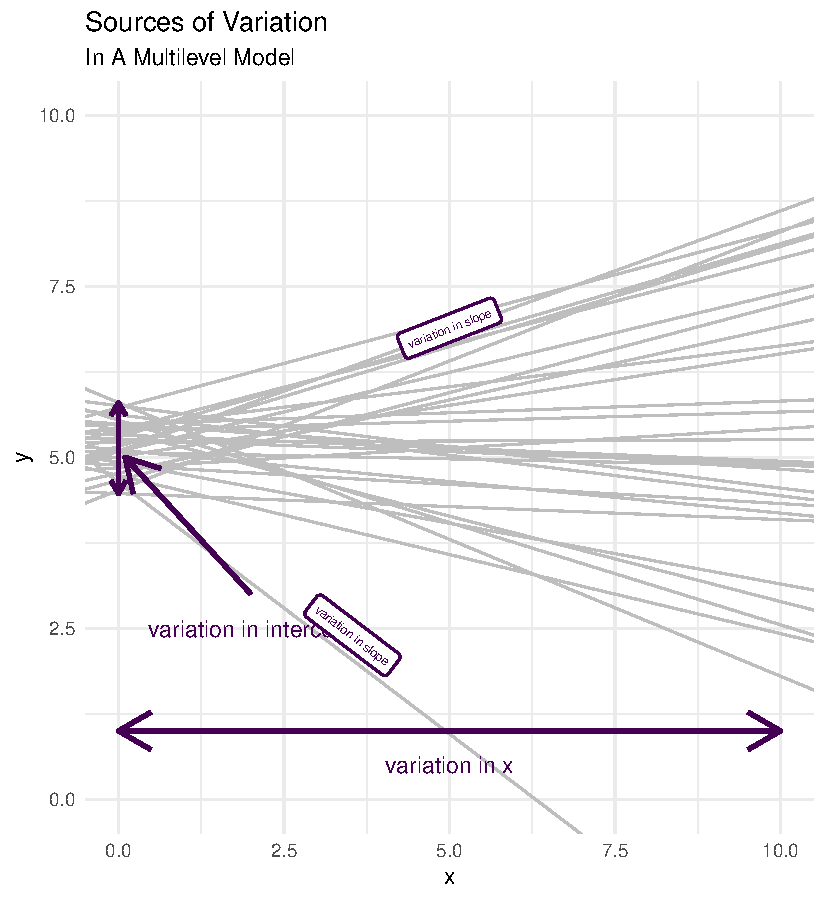
\includegraphics{./cross-sectional_files/figure-pdf/fig-variationsources-1.pdf}

}

\caption{\label{fig-variationsources}Sources of Variation in a
Multilevel Model}

\end{figure}

\hypertarget{variation-in-intercepts-or-outcomes}{%
\subsection{Variation In Intercepts or
Outcomes}\label{variation-in-intercepts-or-outcomes}}

In Equation~\ref{eq-MLMsubstantive2}, \(var(u_{0j})\) is the model
estimated amount of variation in the \emph{outcome}, \(y_{ij}\).

In the regression in Section~\ref{sec-regression}, there is discernible
between country variation, but more of the variation is between
individuals within the same country. Put another way, there is a
moderate tendency for children in families in the same country to have
similar outcomes, but two children in families in the same country may
also have very different outcomes. Children from families in different
countries may be as similar as children from families in the same
country.

\hypertarget{variation-in-predictors}{%
\subsection{Variation In Predictors}\label{variation-in-predictors}}

Equally important, I think, but much less frequently explored than
variation in \emph{outcomes}, is the possibility of variation in
\emph{predictors}. In the substantive example that we have employed so
far, the \emph{predictors} are different \emph{parenting behaviors}, so
considering variation in \emph{predictors} allows us to consider
variation in \emph{parenting behaviors}, as well as variation in the
\emph{outcomes} of those behaviors.

We would estimate variation in behaviors in much the same way that we
would estimate variation in outcomes, estimating an unconditional model,
but substituting \(x\) for \(y\).

\begin{equation}\protect\hypertarget{eq-unconditionalx}{}{x_{ij} = \beta_0 + u_{0j} + e_{ij}}\label{eq-unconditionalx}\end{equation}

Then, similarly, the variation in a predictor attributable to the
clustered nature of the data--in this case the clustering of individuals
in countries--is given by:

\begin{equation}\protect\hypertarget{eq-ICCx}{}{\text{ICC}_x = \frac{var(u_{0j})}{var(u_{0j}) + var(e_{ij})}}\label{eq-ICCx}\end{equation}

\hypertarget{variation-in-slopes}{%
\subsection{Variation in Slopes}\label{variation-in-slopes}}

Another possible type of variation to investigate is variation in the
relationship of \(x\) and \(y\), which is represented in the multilevel
model by examining variation in the \(\beta\)'s.

\hypertarget{variation-as-an-outcome}{%
\subsection{Variation As An Outcome}\label{variation-as-an-outcome}}

Even less common is to examine \emph{variation} itself as an outcome
(Burkner, 2018).

\begin{equation}\protect\hypertarget{eq-distributional}{}{\sigma_{yij} = \beta_0 + \beta_1 x_1 + u_{0j} + e_{ij}}\label{eq-distributional}\end{equation}

Here, the variation in the outcome, \(\sigma_{yij}\), rather than the
mean level of the outcome, \(y_{ij}\), is the focus of interest. My
notation for Equation~\ref{eq-distributional} draws upon Burkner
(2018)'s notation, but is modified in order to be consistent with the
rest of this document.

Why might such models be of conceptual interest? Imagine for example,
that the \emph{variation} in psychological well-being is higher in
countries with higher levels of poverty, or higher levels of income
inequality. The use of such models as this, discussed in more detail by
Burkner (2018), would allow us to explore such a question.

Of note, while I do not explore in detail differences between Bayesian
and frequentist approaches to multilevel modeling in this document,
these models are likely to be only estimable with Bayesian software
rather than with frequentist software (Burkner, 2018).

\hypertarget{maximal-models}{%
\subsection{Maximal Models}\label{maximal-models}}

Hypothetically, one might imagine that there could be group level
unobserved factors which affect regression slopes---i.e.~the
relationship between a predictor x and outcome variable y---arguably,
were one to ignore these unobserved factors in statistical estimation,
they would show up either in an error term, or in the regression
coefficients themselves. Were they to show up in the regression
coefficients this would represent statistical bias and a substantive
mis-estimation of important effects. thus, there is a conceptual
argument for including as many random effects---i.e.~random slopes---in
a statistical model as possible.

Models with all possible random effects are termed \emph{maximal models}
(Barr et al., 2013; Frank, 2018). Such models include a large number of
random slopes, e.g.~\(u_1, u_2, u_3, ..., etc.\) even when some of those
estimated slopes are close to 0. Such models may be more easily
estimable when using Bayesian estimation (Frank, 2018), a topic which I
do not cover in detail in this document.

It should be noted that Matuschek et al. (2017) argue that such a
\emph{maximal} approach may lead to a loss of statistical power and
further argue that one should adhere to ``a random effect structure that
is supported by the data.'' In contrast, Nalborczyk et al. (2019) argue
that maximal models are supported under the Bayesian approach. Oberauer
(2022) also argues for including multiple random slopes. Schielzeth \&
Forstmeier (2009) make a similar argument from a frequentist
perspective.

\hypertarget{sec-wrongapproaches}{%
\section{Some Wrong (or Partially Wrong)
Approaches}\label{sec-wrongapproaches}}

When data are clustered--e.g.~residents in neighborhoods, children in
schools, families in countries--it is worth discussing the fact that we
have several choices statistically as how to proceed, other than using a
multilevel model. Given the discussion so far, we can see the advantages
of a multilevel model over these other approaches:

\begin{enumerate}
\def\labelenumi{\arabic{enumi}.}
\tightlist
\item
  First, we could simply ignore the clustering, and treat the data as
  though it were composed of statistically independent individuals,
  i.e.~statistically independent \(e_i\). As we have discussed above,
  however, this approach has at least two disadvantages. First, as
  discussed in Section~\ref{sec-pvalues}, this approach will
  mis-estimate standard errors, most often underestimating them,
  resulting in underestimated p values and false positives. Second, as
  discussed in Section~\ref{sec-multilevelstructure} ignoring clustering
  runs the risk of estimating regression \(\beta\)'s that are not
  estimated with information about the multilevel structure of the data,
  with the possibility that \(\beta\) coefficients may not only have
  incorrect statistical significance, but also incorrect magnitude, and
  even incorrect sign.
\item
  A second approach would be to \emph{aggregate} the data to the level
  of the higher social unit, e.g.~aggregating the data at the level of
  the neighborhood. Here we run into an idea similar to that discussed
  in Section~\ref{sec-multilevelstructure}, the ``ecological fallacy'':
  the idea that group level and individual level relationships are
  necessarily the same (Firebaugh, 2001).
\item
  Lastly, we could adopt a statistical strategy of \emph{clustering} the
  standard errors. Clustering the standard errors means that standard
  errors are corrected for the non-independence of the \(e_i\) within
  clusters. Thus, \emph{p} values are estimated correctly. However,
  clustering still does not account for the multilevel structure of the
  data (Section~\ref{sec-multilevelstructure}), and thus when
  relationships between \emph{x}'s and \emph{y} at different levels of
  the data are very different, simply clustering the standard errors may
  not give correct estimates of the \(\beta\)'s.
\end{enumerate}

\bookmarksetup{startatroot}

\hypertarget{the-longitudinal-multilevel-model}{%
\chapter{The Longitudinal Multilevel
Model}\label{the-longitudinal-multilevel-model}}

\begin{Shaded}
\begin{Highlighting}[]
\FunctionTok{library}\NormalTok{(haven) }\CommentTok{\# read Stata}

\FunctionTok{library}\NormalTok{(tibble) }\CommentTok{\# data frames}

\FunctionTok{library}\NormalTok{(ggplot2) }\CommentTok{\# beautiful graphs}

\FunctionTok{library}\NormalTok{(geomtextpath) }\CommentTok{\# path geoms}

\FunctionTok{library}\NormalTok{(dplyr) }\CommentTok{\# data wrangling}
\end{Highlighting}
\end{Shaded}

\begin{verbatim}

Attaching package: 'dplyr'
\end{verbatim}

\begin{verbatim}
The following objects are masked from 'package:stats':

    filter, lag
\end{verbatim}

\begin{verbatim}
The following objects are masked from 'package:base':

    intersect, setdiff, setequal, union
\end{verbatim}

\begin{Shaded}
\begin{Highlighting}[]
\FunctionTok{library}\NormalTok{(tidyr) }\CommentTok{\# data tidying}

\FunctionTok{library}\NormalTok{(pander) }\CommentTok{\# nice tables}

\CommentTok{\# library(gt) \# beautiful tables}
\end{Highlighting}
\end{Shaded}

\begin{quote}
``Mathematics is the art of giving the same name to different things.''
(Poincare, 1908)
\end{quote}

Counter-intuitively, and surprisingly, the mathematics of estimating
models with cross-sectional clustered data easily generalizes to
longitudinal data. In cross sectional clustered data, we imagine
\emph{individuals clustered in neighborhoods, schools, or countries}.

\hypertarget{tbl-levelscrosssectional}{}
\begin{longtable}[]{@{}ll@{}}
\caption{\label{tbl-levelscrosssectional}Levels in Cross-Sectional
Data}\tabularnewline
\toprule()
Level & Example(s) \\
\midrule()
\endfirsthead
\toprule()
Level & Example(s) \\
\midrule()
\endhead
1 & Individuals \\
2 & Schools \\
& Neighborhoods \\
& Countries \\
\bottomrule()
\end{longtable}

In longitudinal data, we consider the \emph{first level} to be that of
\emph{time points}, or \emph{study waves}, which we sometimes call the
\emph{person-observation}. The \emph{second level} is then the
individual.

\hypertarget{tbl-levelslongitudinal}{}
\begin{longtable}[]{@{}ll@{}}
\caption{\label{tbl-levelslongitudinal}Levels in Longitudinal
Data}\tabularnewline
\toprule()
Level & Example(s) \\
\midrule()
\endfirsthead
\toprule()
Level & Example(s) \\
\midrule()
\endhead
1 & Timepoints \\
2 & Individuals \\
\bottomrule()
\end{longtable}

While it is less common, we could then easily add additional clustering
to this longitudinal model, for example, clustering of individuals
inside social units.

\hypertarget{tbl-levelslongitudinal2}{}
\begin{longtable}[]{@{}ll@{}}
\caption{\label{tbl-levelslongitudinal2}Multiple Levels in Longitudinal
Data}\tabularnewline
\toprule()
Level & Example(s) \\
\midrule()
\endfirsthead
\toprule()
Level & Example(s) \\
\midrule()
\endhead
1 & Timepoints \\
2 & Individuals \\
3 & Schools \\
& Neighborhoods \\
& Countries \\
\bottomrule()
\end{longtable}

\hypertarget{use-data-with-multiple-observations-per-individual}{%
\section{Use Data With Multiple Observations Per
Individual}\label{use-data-with-multiple-observations-per-individual}}

Multilevel data suitable for longitudinal analysis therefore has
\emph{multiple rows of data per individual}. Put another way,
\emph{every row of data is a person-timepoint}.

\begin{quote}
This method of organizing data is known as the \emph{long} format.
Another way of organizing longitudinal data--which I do not discuss in
detail here--is the \emph{wide} format in which every individual still
has only one row of data. In \emph{wide} data, the different timepoints
are in different columns of data.
\end{quote}

\hypertarget{tbl-datalong}{}
\begin{longtable}[]{@{}lll@{}}
\caption{\label{tbl-datalong}Data in Long Format}\tabularnewline
\toprule()
id & t & x \\
\midrule()
\endfirsthead
\toprule()
id & t & x \\
\midrule()
\endhead
1 & 1 & 10 \\
1 & 2 & 20 \\
1 & 3 & 30 \\
2 & 1 & 20 \\
2 & 2 & 30 \\
2 & 3 & 40 \\
\bottomrule()
\end{longtable}

\hypertarget{tbl-datawide}{}
\begin{longtable}[]{@{}llll@{}}
\caption{\label{tbl-datawide}Data in Wide Format}\tabularnewline
\toprule()
id & x1 & x2 & x3 \\
\midrule()
\endfirsthead
\toprule()
id & x1 & x2 & x3 \\
\midrule()
\endhead
1 & 10 & 20 & 30 \\
2 & 20 & 30 & 40 \\
\bottomrule()
\end{longtable}

\begin{Shaded}
\begin{Highlighting}[]
\NormalTok{simulated\_multilevel\_longitudinal\_data }\OtherTok{\textless{}{-}} 
  \FunctionTok{read\_dta}\NormalTok{(}\StringTok{"./simulate{-}and{-}analyze{-}multilevel{-}data/simulated\_multilevel\_longitudinal\_data.dta"}\NormalTok{)}
\end{Highlighting}
\end{Shaded}

\begin{Shaded}
\begin{Highlighting}[]
\NormalTok{pander}\SpecialCharTok{::}\FunctionTok{pander}\NormalTok{(}\FunctionTok{head}\NormalTok{(simulated\_multilevel\_longitudinal\_data))}
\end{Highlighting}
\end{Shaded}

\hypertarget{tbl-simulatedlongitudinaldata}{}
\begin{longtable}[]{@{}
  >{\centering\arraybackslash}p{(\columnwidth - 12\tabcolsep) * \real{0.0694}}
  >{\centering\arraybackslash}p{(\columnwidth - 12\tabcolsep) * \real{0.1250}}
  >{\centering\arraybackslash}p{(\columnwidth - 12\tabcolsep) * \real{0.3056}}
  >{\centering\arraybackslash}p{(\columnwidth - 12\tabcolsep) * \real{0.1389}}
  >{\centering\arraybackslash}p{(\columnwidth - 12\tabcolsep) * \real{0.1389}}
  >{\centering\arraybackslash}p{(\columnwidth - 12\tabcolsep) * \real{0.0556}}
  >{\centering\arraybackslash}p{(\columnwidth - 12\tabcolsep) * \real{0.1389}}@{}}
\caption{\label{tbl-simulatedlongitudinaldata}Simulated Longitudinal
Multilevel Data}\tabularnewline
\toprule()
\begin{minipage}[b]{\linewidth}\centering
id
\end{minipage} & \begin{minipage}[b]{\linewidth}\centering
warmth
\end{minipage} & \begin{minipage}[b]{\linewidth}\centering
physical\_punishment
\end{minipage} & \begin{minipage}[b]{\linewidth}\centering
country
\end{minipage} & \begin{minipage}[b]{\linewidth}\centering
outcome
\end{minipage} & \begin{minipage}[b]{\linewidth}\centering
t
\end{minipage} & \begin{minipage}[b]{\linewidth}\centering
x\_noise
\end{minipage} \\
\midrule()
\endfirsthead
\toprule()
\begin{minipage}[b]{\linewidth}\centering
id
\end{minipage} & \begin{minipage}[b]{\linewidth}\centering
warmth
\end{minipage} & \begin{minipage}[b]{\linewidth}\centering
physical\_punishment
\end{minipage} & \begin{minipage}[b]{\linewidth}\centering
country
\end{minipage} & \begin{minipage}[b]{\linewidth}\centering
outcome
\end{minipage} & \begin{minipage}[b]{\linewidth}\centering
t
\end{minipage} & \begin{minipage}[b]{\linewidth}\centering
x\_noise
\end{minipage} \\
\midrule()
\endhead
1 & 129.6 & 84.86 & 15 & 685.3 & 1 & 2.872 \\
1 & 124.1 & 84.86 & 15 & 675.8 & 2 & -12.67 \\
1 & 126.9 & 84.86 & 15 & 691.2 & 3 & -19.88 \\
2 & 106.2 & 90.91 & 24 & 330.5 & 1 & -6.262 \\
2 & 128.3 & 90.91 & 24 & 479.6 & 2 & 5.793 \\
2 & 142.2 & 90.91 & 24 & 580.6 & 3 & 9.695 \\
\bottomrule()
\end{longtable}

\begin{Shaded}
\begin{Highlighting}[]
\NormalTok{simulated\_multilevel\_longitudinal\_data }\SpecialCharTok{\%\textgreater{}\%}
  \FunctionTok{slice\_head}\NormalTok{(}\AttributeTok{n =} \DecValTok{30}\NormalTok{) }\SpecialCharTok{\%\textgreater{}\%} 
  \FunctionTok{ggplot}\NormalTok{(}\FunctionTok{aes}\NormalTok{(}\AttributeTok{x =}\NormalTok{ t,}
           \AttributeTok{y =}\NormalTok{ outcome,}
           \AttributeTok{color =} \FunctionTok{factor}\NormalTok{(id))) }\SpecialCharTok{+}
  \CommentTok{\# geom\_point() +}
  \FunctionTok{geom\_smooth}\NormalTok{(}\AttributeTok{method =} \StringTok{"lm"}\NormalTok{, }\AttributeTok{se =} \ConstantTok{FALSE}\NormalTok{) }\SpecialCharTok{+}
  \FunctionTok{scale\_color\_viridis\_d}\NormalTok{(}\AttributeTok{name =} \StringTok{"individual"}\NormalTok{) }\SpecialCharTok{+}
  \FunctionTok{labs}\NormalTok{(}\AttributeTok{title =} \StringTok{"Desirable Outcome by Time"}\NormalTok{,}
       \AttributeTok{subtitle =} \StringTok{"By Individual"}\NormalTok{,}
       \AttributeTok{caption =} \StringTok{"Simulated Longitudinal Data; Selected Individuals"}\NormalTok{,}
       \AttributeTok{x =} \StringTok{"time"}\NormalTok{,}
       \AttributeTok{y =} \StringTok{"desirable outcome"}\NormalTok{) }\SpecialCharTok{+}
  \FunctionTok{theme\_minimal}\NormalTok{() }\SpecialCharTok{+}
  \FunctionTok{theme}\NormalTok{(}\AttributeTok{legend.position =} \StringTok{"none"}\NormalTok{)}
\end{Highlighting}
\end{Shaded}

\begin{verbatim}
`geom_smooth()` using formula = 'y ~ x'
\end{verbatim}

\begin{figure}[H]

{\centering 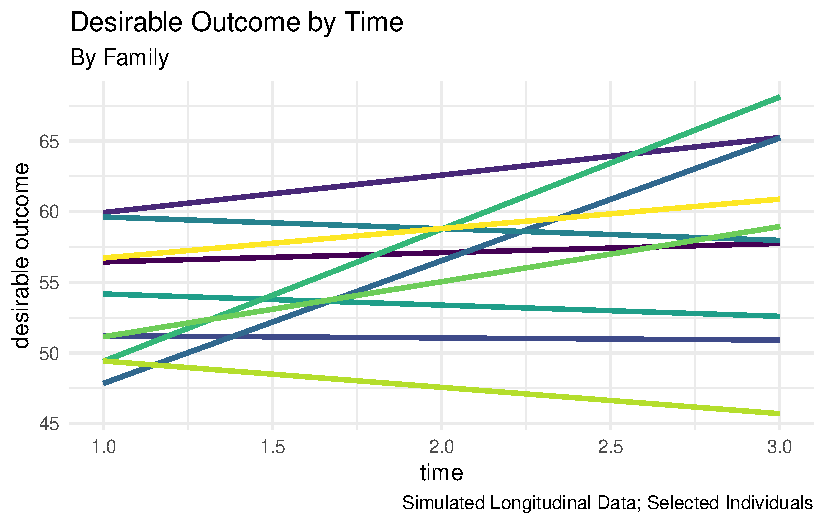
\includegraphics{./longitudinal_files/figure-pdf/fig-data2-1.pdf}

}

\caption{\label{fig-data2}Graph of Simulated Longitudinal Data}

\end{figure}

\hypertarget{the-equation-1}{%
\section{The Equation}\label{the-equation-1}}

When data are in \emph{long} format, the following equation is
applicable.

\begin{equation}\protect\hypertarget{eq-MLM-longitudinal}{}{\text{outcome}_{itj} = \beta_0 + \beta_1 \text{parental warmth}_{itj} + \beta_2 \text{physical punishment}_{itj} + \beta_3 \text{time}_{itj} \ + }\label{eq-MLM-longitudinal}\end{equation}

\[u_{0j} + u_{1j} \times \text{parental warmth}_i \ + \]
\[v_{0i} + v_{1i} \times t + e_{ij}\] Here I include a random slope
(\(u_{1j}\)) at the country level for parental warmth, as well as a
random slope (\(v_{1j}\)) at the individual level for time.

\hypertarget{sec-regressionlongitudinal}{%
\section{Regression With Simulated Multi-Country Longitudinal
Data}\label{sec-regressionlongitudinal}}

The Stata command that we use to analyze this data is:

\texttt{mixed\ outcome\ t\ warmth\ physical\_punishment\ \textbar{}\textbar{}\ country:\ warmth\ \textbar{}\textbar{}\ id:\ t}

\begin{longtable}[]{@{}lll@{}}
\toprule()
& longitudinal & \\
\midrule()
\endhead
t & 4.124 & ** \\
warmth & 4.874 & ** \\
physical\_punishment & -3.054 & ** \\
Intercept & 5.860 & \\
var(warmth) & 0.890 & \\
var(\_cons) & 415.073 & \\
var(\_cons) & 0.000 & \\
var(t) & 0.000 & \\
var(e) & 2660.874 & \\
\bottomrule()
\end{longtable}

** p\textless.01, * p\textless.05

Examining the regression results, the results of the model suggest that
child outcomes improve over time. Better child outcomes are again
associated with parental warmth, and parental use of physical punishment
is associated with reduced child outcomes.

\hypertarget{autocorrelation}{%
\section{Autocorrelation}\label{autocorrelation}}

When data are ordered by a time variable \(t\), it is possible that
observations that are closer together in time will have a higher
correlation than observations that are distant in time. In the simplest
example, \(e_{i, t=k}\) may be correlated with \(e_{i, t=k-1}\). This
phenomenon is known as \emph{autocorrelation}. As Hooper (2022) would
suggest, it may make sense to assume that the correlation between
observations ``decays with increasing separation in time''.

Most software programs for multilevel modeling allow one to incorporate
measures of autocorrelation so that, e.g., \(e_{i,t=3}\) is allowed to
be correlated with \(e_{i,t=2}\), which in turn can be correlated with
\(e_{i,t=1}\). More complex autocorrelation structures are usually also
possible (StataCorp, 2021a).

\hypertarget{causality}{%
\section{Causality}\label{causality}}

\hypertarget{the-importance-of-causal-reasoning}{%
\subsection{The Importance of Causal
Reasoning}\label{the-importance-of-causal-reasoning}}

Causal reasoning is sometimes considered to be a statistical--or even
overly technical--concern. Arguably, however, whenever one is using
research to make recommendations about interventions, or treatments, or
policies, one is engaging in some form of causal reasoning (Duncan \&
Gibson-Davis, 2006).

\begin{quote}
If one is saying that implementing \emph{x} would result in beneficial
changes in \emph{y}, one is arguing--at least implicitly--that \emph{x}
is one of the causes of \emph{y}.
\end{quote}

It then behooves one to be explicit about this chain of causal
reasoning. For example, to continue one of the substantive examples of
this document, if one is going to argue for programs, interventions, or
treatments that promote \emph{parental warmth}, or that discourage
parental use of \emph{physical punishment} with the aim of improving
children's \emph{mental health}, one must be at least reasonably sure
that \emph{parental warmth} and \emph{physical punishment} are
\emph{causes} of children's mental health.

Randomized studies provide the best evidence about the internal validity
of causal relationships. However, randomized studies have certain
limitations (Diener et al., 2022). First of all--especially in a study
with a smaller sample--randomization may not always be perfect, and the
control and treatment groups may not be statistically equivalent.
Secondly, because of ethical concerns some studies can not be conducted
with randomization (Diener et al., 2022). For example, in the study of
parenting and child development, children cannot ethically be assigned
to parents with different styles of parenting and followed over the long
term. Thus, methods that provide rigorous causal estimation with
observational methods are necessary (Diener et al., 2022).

Because of the assumed superiority of studies that employ randomization,
it is sometimes maintained that \emph{correlation is not causation} and
that studies that do not make use of randomization are \emph{only
observational} and \emph{correlational}, and that results from
observational studies cannot be used to support causal conclusions.
However, in an important review (Waddington et al., 2022) suggested that
studies using appropriately quantitative methods can provide causally
robust conclusions.

In a statement salient for social research, Duncan \& Gibson-Davis
(2006) point out the logical inconsistency of writing that does not
rigorously address causal processes, but then goes on to suggest
interventions or treatment or policies:

\begin{quote}
``Developmental studies are usually careful to point out when their data
do not come from a randomized experiment. As with much of the
nonexperimental literature in developmental psychology, most of the
articles then go on to assert that, as a consequence, it is impossible
to draw causal inferences from the analysis. Indeed, much of their
language describing results is couched in terms of `associations'
between child care quality and child outcomes. It is not uncommon,
however, to see these papers make explicit statements about effects, and
others draw explicit policy conclusions. For instance, NICHD (1997, 876)
stated, `The interaction analyses provided evidence that high-quality
child care served a compensatory function for children whose maternal
care was lacking.' On the policy side, NICHD (2002c, 199) asserted,
`These findings provide empirical support for policies that improve
state regulations for caregiver training and child-staff ratios.'\,''
\end{quote}

\begin{quote}
``One cannot have it both ways. Studies that do not aspire to causal
analysis should make no claim whatsoever about effects and draw no
policy conclusions. At the same time, it would be a terrible waste of
resources to conduct expensive longitudinal studies without attempting
to use them for causal modeling.''
\end{quote}

Lastly, because of their often small samples, randomized studies may
have high internal validity, but much lower external validity, or
generalization to larger populations (Diener et al., 2022). This issue
of generalizability becomes increasingly salient, when we are reminded
of the fact that so little social and psychological research has been
conducted outside of North American contexts (Draper et al., 2022;
Henrich et al., 2010). It is necessary to make use of broadly
representative observational data sets, and appropriately sophisticiated
quantitative methods to make causally robust conclusions from
observational data.

\hypertarget{formal-criteria-of-causality}{%
\subsection{Formal Criteria of
Causality}\label{formal-criteria-of-causality}}

For x to be a cause of y, one needs the following 3 things to be true
(Holland, 1986).

\begin{enumerate}
\def\labelenumi{\arabic{enumi}.}
\tightlist
\item
  \emph{x} is (are) associated with (correlated with) \emph{y}.
\item
  \emph{x} come(s) before \emph{y} in time.
\item
  \emph{z}--or other factors--cannot explain the association of
  (correlation of) \emph{x} and \emph{y}.
\end{enumerate}

\begin{Shaded}
\begin{Highlighting}[]
\NormalTok{DiagrammeR}\SpecialCharTok{::}\FunctionTok{grViz}\NormalTok{(}\StringTok{"}

\StringTok{digraph G \{}

\StringTok{rankdir=\textquotesingle{}LR\textquotesingle{}}

\StringTok{x {-}\textgreater{} y}
\StringTok{z {-}\textgreater{} y}
\StringTok{z {-}\textgreater{} x [dir=\textquotesingle{}both\textquotesingle{}]}

\StringTok{\} }
\StringTok{"}\NormalTok{, }\AttributeTok{height =} \StringTok{\textquotesingle{}100\%\textquotesingle{}}\NormalTok{)}
\end{Highlighting}
\end{Shaded}

\begin{figure}

{\centering 

}

\caption{\label{fig-causality}Formal Criteria of Causality}

\end{figure}

\begin{quote}
If \emph{z} is omitted from the regression model, then the estimates for
\(x \rightarrow y\) (i.e.~\(\beta_{x \rightarrow y}\)) will be biased.
In the most common scenario \(\beta_{x \rightarrow y}\) will likely be
an over-estimate of the effect, and statistical significance of
\(\beta_{x \rightarrow y}\) may represent a false positive.
\end{quote}

It is likely useful to restate the above abstract statements in terms of
the substantive issues that I have been considering so far in this
document.

For \emph{parenting} to be a cause of \emph{child outcomes}, one needs
the following 3 things to be true (Holland, 1986).

\begin{enumerate}
\def\labelenumi{\arabic{enumi}.}
\tightlist
\item
  \emph{parenting} is (are) associated with (correlated with)
  \emph{child outcomes}.
\item
  \emph{parenting} come(s) before \emph{child outcomes} in time.
\item
  \emph{SES}, \emph{community characteristics}--or other factors--cannot
  explain the association of (correlation of) \emph{parenting} and
  \emph{child outcomes}.
\end{enumerate}

\begin{Shaded}
\begin{Highlighting}[]
\NormalTok{DiagrammeR}\SpecialCharTok{::}\FunctionTok{grViz}\NormalTok{(}\StringTok{"}

\StringTok{digraph G \{}

\StringTok{rankdir=\textquotesingle{}LR\textquotesingle{}}

\StringTok{x [label = \textquotesingle{}parenting\textquotesingle{}]}
\StringTok{y [label = \textquotesingle{}child outcome\textquotesingle{}]}
\StringTok{z [label = \textquotesingle{}other factors\textquotesingle{}]}

\StringTok{x {-}\textgreater{} y}
\StringTok{z {-}\textgreater{} y}
\StringTok{z {-}\textgreater{} x [dir=\textquotesingle{}both\textquotesingle{}]}

\StringTok{\} }
\StringTok{"}\NormalTok{, }\AttributeTok{height =} \StringTok{\textquotesingle{}100\%\textquotesingle{}}\NormalTok{)}
\end{Highlighting}
\end{Shaded}

\begin{figure}

{\centering 

}

\caption{\label{fig-causalitysubstantive}Formal Criteria of Causality}

\end{figure}

If \emph{other factors} are omitted from the regression model, then the
estimates for \(\text{parenting} \rightarrow \text{child outcome}\)
(i.e.~\(\beta_{\text{parenting} \rightarrow \text{child outcome}}\))
will be biased. In the most common scenario
\(\beta_{\text{parenting} \rightarrow \text{child outcome}}\) will
likely be an over-estimate of the effect, and statistical significance
of \(\beta_{\text{parenting} \rightarrow \text{child outcome}}\) may
represent a false positive.

\hypertarget{simpsons-paradox}{%
\subsection{Simpson's Paradox}\label{simpsons-paradox}}

Earlier, in Section~\ref{sec-multilevelstructure}, I referred to the
idea of \emph{multilevel structure} wherein failure to account for the
clustering of data--omission of \(u_0\) from the equation being
estimated--may lead to incorrect conclusions. A closely related
phenomenon is that of \emph{Simpson's Paradox} (Simpson, 1951) wherein
omission of a relevant \emph{covariate} (e.g.~SES, community
characteristics, country level characteristics) may also lead to
dramatically incorrect results.

Statistically, we imagine a situation where the true model is:

\[\text{child outcome}_{it} = \beta_0 + \beta_1 \text{parenting}_{it} + \beta_2 \text{community or country characteristic}_{it} + e_{it}\]
If \emph{community or country characteristics} in fact influence
\emph{outcome}, but are not included in the statistical model, perhaps
because they are not measured in the data, then the estimate of
\(\beta_1\) for \emph{parenting} will be biased. See
Figure~\ref{fig-Simpson} for an illustration.

\begin{Shaded}
\begin{Highlighting}[]
\NormalTok{multilevelstructure }\OtherTok{\textless{}{-}}
  \FunctionTok{read\_dta}\NormalTok{(}\StringTok{"./simulate{-}and{-}analyze{-}multilevel{-}data/multilevelstructure.dta"}\NormalTok{)}

\NormalTok{multilevelstructure}\SpecialCharTok{$}\NormalTok{country }\OtherTok{\textless{}{-}} \FunctionTok{factor}\NormalTok{(multilevelstructure}\SpecialCharTok{$}\NormalTok{country)}
\end{Highlighting}
\end{Shaded}

\begin{Shaded}
\begin{Highlighting}[]
\FunctionTok{ggplot}\NormalTok{(multilevelstructure, }
             \FunctionTok{aes}\NormalTok{(}\AttributeTok{x =}\NormalTok{ x,}
                 \AttributeTok{y =}\NormalTok{ y)) }\SpecialCharTok{+}
  \FunctionTok{geom\_smooth}\NormalTok{(}\AttributeTok{method =} \StringTok{"lm"}\NormalTok{) }\SpecialCharTok{+}
  \FunctionTok{geom\_point}\NormalTok{(}\FunctionTok{aes}\NormalTok{(}\AttributeTok{color =}\NormalTok{ country)) }\SpecialCharTok{+} \CommentTok{\# points with country color}
  \FunctionTok{geom\_smooth}\NormalTok{(}\FunctionTok{aes}\NormalTok{(}\AttributeTok{color =}\NormalTok{ country), }\CommentTok{\# smoothers with country color}
              \AttributeTok{method =} \StringTok{"lm"}\NormalTok{) }\SpecialCharTok{+} 
  \FunctionTok{labs}\NormalTok{(}\AttributeTok{title =} \StringTok{"Desirable Outcome as a Function of Intervention or Treatment"}\NormalTok{,}
       \AttributeTok{x =} \StringTok{"intervention or treatment or parenting (x)"}\NormalTok{,}
       \AttributeTok{y =} \StringTok{"desirable outcome (y)"}\NormalTok{,}
       \AttributeTok{caption =} \StringTok{"Slope not accounting for covariate(s) slopes downward. }\SpecialCharTok{\textbackslash{}n}\StringTok{Slope accounting for covariate(s) slopes upward."}\NormalTok{) }\SpecialCharTok{+}
  \FunctionTok{scale\_color\_viridis\_d}\NormalTok{(}\AttributeTok{name =} \StringTok{"covariate (z)"}\NormalTok{) }\SpecialCharTok{+}
  \FunctionTok{theme\_minimal}\NormalTok{() }
\end{Highlighting}
\end{Shaded}

\begin{verbatim}
`geom_smooth()` using formula = 'y ~ x'
`geom_smooth()` using formula = 'y ~ x'
\end{verbatim}

\begin{figure}[H]

{\centering 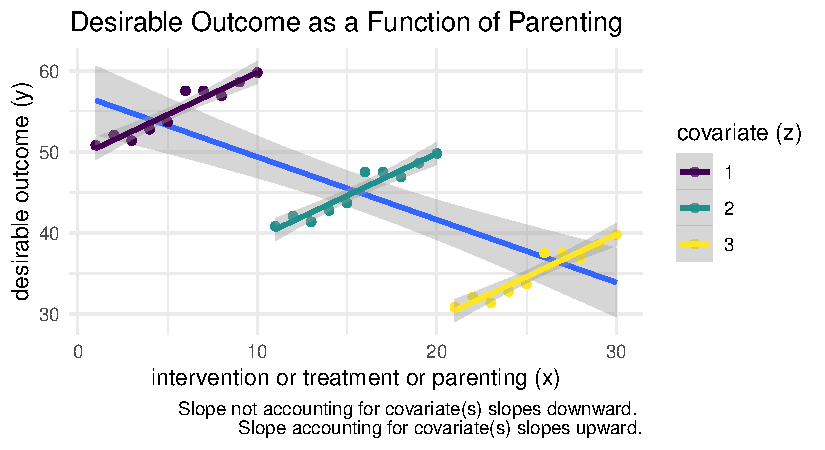
\includegraphics{./longitudinal_files/figure-pdf/fig-Simpson-1.pdf}

}

\caption{\label{fig-Simpson}An Illustration of Simpson's Paradox}

\end{figure}

\hypertarget{a-simpler-multilevel-model-to-explore-causality}{%
\subsection{A Simpler Multilevel Model To Explore
Causality}\label{a-simpler-multilevel-model-to-explore-causality}}

For purposes of explication of ideas about causal estimation, in this
section, I imagine a simpler equation where I am only considering the
clustering of \emph{person timepoints} within \emph{individual people},
and ignoring for the moment--again for the sake of exposition--the
clustering of \emph{individuals} within \emph{countries}.

After explication and comprehension of this model, however, it is a
simple matter to add back in the random effects for country level
clustering.

The appropriate multilevel model is below.

\begin{equation}\protect\hypertarget{eq-MLM-simpler}{}{\text{outcome}_{it} = \beta_0 + \beta_1 \text{parental warmth}_{it} + \beta_2 \text{physical punishment}_{it} + \beta_3 \text{time}_{it} \ + }\label{eq-MLM-simpler}\end{equation}

\[v_{0i} + e_{it}\]

Note that in Equation~\ref{eq-MLM-simpler}, if one were estimating a
\emph{multilevel model}, one would consider the \(v_{0i}\) to be a
randomly varying parameter with a mean of 0, and a variance of
\(\sigma^2(v_{0i})\).

\hypertarget{fixed-effects-regression}{%
\subsection{Fixed Effects Regression}\label{fixed-effects-regression}}

I can use the same equation:

\begin{equation}\protect\hypertarget{eq-FE}{}{\text{outcome}_{it} = \beta_0 + \beta_1 \text{parental warmth}_{it} + \beta_2 \text{physical punishment}_{it} + \beta_3 \text{time}_{it} \ + }\label{eq-FE}\end{equation}

\[v_{0i} + e_{it}\]

However, in Equation~\ref{eq-FE}, I now consider the \(v_{0i}\) to be
\emph{estimable} for each individual \(i\) in the data. In effect, the
\(v_{0i}\) become a unique indicator variable for each individual in the
data set. This is known as a \emph{fixed effects regression model}.

Details are provided in Allison (2009) and Wooldridge (2010). StataCorp
(2021b) provides an exceptionally clear explication of the core idea of
fixed effects regression. The essential idea is that the fixed effects
model provides statistical control for all time invariant
characteristics of study participants, such as--as is often the case in
many data sets--their racial or ethnic identity, or neighborhood of
residence, or other characteristics which by definition are time
invariant, such as the region of the country or city in which a
respondent was born.

Thus, by ruling out many potential confounds, fixed effects regression
methods provide much more causally robust analyses, specifically because
they control for many more possible confounding variables than do
standard regression methods, including multilevel models, which are only
able to control for the variables that are measured in the study
\textbf{and} included within the regression model.

However, a disadvantage of the fixed effects approach is that this
approach can not provide estimates for any time invariant characteristic
of study participants. Indeed, if one includes time invariant variables
into a fixed effects regression, they are automatically dropped from the
regression results as can be seen in the regression table below.

The relevant Stata commands are:

\begin{itemize}
\tightlist
\item
  \texttt{mixed\ outcome\ t\ warmth\ physical\_punishment\ \textbar{}\textbar{}\ id:}
\item
  \texttt{xtreg\ outcome\ t\ warmth\ physical\_punishment,\ i(id)\ fe}
\end{itemize}

\begin{longtable}[]{@{}lllll@{}}
\toprule()
& MLM & & FE & \\
\midrule()
\endhead
t & 3.710 & * & 4.093 & * \\
warmth & 4.921 & ** & 4.883 & ** \\
physical\_punishment & -3.330 & ** & & \\
Intercept & 29.811 & & -298.721 & ** \\
var(\_cons) & 11955.673 & & & \\
var(e) & 2874.374 & & & \\
Number of observations & & & 3000 & \\
\bottomrule()
\end{longtable}

** p\textless.01, * p\textless.05

\hypertarget{the-correlated-random-effects-model}{%
\subsection{The Correlated Random Effects
Model}\label{the-correlated-random-effects-model}}

The \emph{correlated random effects} model is based upon ideas first
developed by Mundlak (1978) and later explicated in Wooldridge (2010).
Antonakis et al. (2021) and Schunck (2013) provide very intuitive
explanations of this model.

The central idea is that one can obtain estimates of both the time
invariant variables, and estimates for time varying variables. The key
idea is that for time varying variables, I include the individual level
mean for that variable in the model. Thus, in the example below, I
include \(\beta_{1a}\overline{\text{parental warmth}}_{i}\).

\begin{equation}\protect\hypertarget{eq-CRE}{}{\text{outcome}_{it} = \beta_0 + \beta_1 \text{parental warmth}_{it} + \beta_{1a}\overline{\text{parental warmth}}_{i} \ + }\label{eq-CRE}\end{equation}

\[\beta_2 \text{physical punishment}_{it} + \beta_3 \text{time}_{it} \ + \]

\[v_{0i} + e_{ij}\]

By including this parameter, I obtain estimates for the time varying
variables that are \emph{equivalent} to what I would obtain from a fixed
effects regression (Schunck, 2013).

The Stata command for the correlated random effects model is:

\texttt{mixed\ outcome\ t\ warmth\ mean\_warmth\ physical\_punishment\ \textbar{}\textbar{}\ id:}

\begin{longtable}[]{@{}
  >{\raggedright\arraybackslash}p{(\columnwidth - 12\tabcolsep) * \real{0.3529}}
  >{\raggedright\arraybackslash}p{(\columnwidth - 12\tabcolsep) * \real{0.1618}}
  >{\raggedright\arraybackslash}p{(\columnwidth - 12\tabcolsep) * \real{0.0588}}
  >{\raggedright\arraybackslash}p{(\columnwidth - 12\tabcolsep) * \real{0.1471}}
  >{\raggedright\arraybackslash}p{(\columnwidth - 12\tabcolsep) * \real{0.0588}}
  >{\raggedright\arraybackslash}p{(\columnwidth - 12\tabcolsep) * \real{0.1618}}
  >{\raggedright\arraybackslash}p{(\columnwidth - 12\tabcolsep) * \real{0.0588}}@{}}
\toprule()
\begin{minipage}[b]{\linewidth}\raggedright
\end{minipage} & \begin{minipage}[b]{\linewidth}\raggedright
MLM
\end{minipage} & \begin{minipage}[b]{\linewidth}\raggedright
\end{minipage} & \begin{minipage}[b]{\linewidth}\raggedright
FE
\end{minipage} & \begin{minipage}[b]{\linewidth}\raggedright
\end{minipage} & \begin{minipage}[b]{\linewidth}\raggedright
CRE
\end{minipage} & \begin{minipage}[b]{\linewidth}\raggedright
\end{minipage} \\
\midrule()
\endhead
t & 3.710 & * & 4.093 & * & 4.093 & * \\
warmth & 4.921 & ** & 4.883 & ** & 4.883 & ** \\
physical\_punishment & -3.330 & ** & & & -3.345 & ** \\
mean\_warmth & & & & & 0.295 & \\
Intercept & 29.811 & & -298.721 & ** & 2.219 & \\
var(\_cons) & 11955.673 & & & & 11946.798 & \\
var(e) & 2874.374 & & & & 2874.229 & \\
Number of observations & & & 3000 & & & \\
\bottomrule()
\end{longtable}

** p\textless.01, * p\textless.05

\bookmarksetup{startatroot}

\hypertarget{conclusion}{%
\chapter{Conclusion}\label{conclusion}}

Many data sets relevant to the study of important social issues, or
social problems, are inherently multilevel. For example, data on diverse
children in schools, diverse individuals in neighborhoods, and
individuals or families in diverse and different countries all have
multilevel structures in which individuals are clustered in higher level
social structures. Data with repeated measures, sometimes termed panel
data, can also be thought of as multilevel data sets, wherein individual
timepoints are nested inside individuals, who may in turn be nested or
clustered in larger social units such as countries. Failure to use
appropriate basic multilevel models with such multilevel data can lead
to answers that are either biased, or demonstrably wrong. Simple
multilevel models allow the researcher to correctly estimate statistical
significance, and to correctly estimate regression coefficients while
accounting for multilevel structure. More advanced applications of
multilevel models allow the researcher to explore the variation in both
predictors and outcomes--and the relationship of predictors to
outcomes--and to characterize the extent of this variation. Lastly,
multilevel models provide a foundation for thinking about closely
related models--fixed effects regression, and correlated random effects
models--that provide methods for estimation that afford stronger causal
conclusions. Thus, for applied researchers, interested in addressing a
variety of social problems and social issues with diverse samples of
individuals, multilevel models present a method to think clearly about
variation, to explore that variation, and to extend that thinking about
variation to estimate more causally robust models within the context of
diversity and variation.

\bookmarksetup{startatroot}

\hypertarget{references}{%
\chapter*{References}\label{references}}
\addcontentsline{toc}{chapter}{References}

\markboth{References}{References}

\hypertarget{refs}{}
\begin{CSLReferences}{1}{0}
\leavevmode\vadjust pre{\hypertarget{ref-Abelson1995}{}}%
Abelson, R. P. (1995). Statistics as principled argument. In
\emph{Statistics as principled argument.} (pp. 221, xv, 221--xv).
Lawrence Erlbaum Associates, Inc.

\leavevmode\vadjust pre{\hypertarget{ref-Allison2009}{}}%
Allison, P. (2009). \emph{Fixed effects regression models}. Sage
Publishing.

\leavevmode\vadjust pre{\hypertarget{ref-Antonakis2019}{}}%
Antonakis, J., Bastardoz, N., \& Ronko, M. (2021). On ignoring the
random effects assumption in multilevel models: Review, critique, and
recommendations. \emph{Organizational Research Methods}, \emph{24},
443--483. \url{https://doi.org/10.1177/1094428119877457}

\leavevmode\vadjust pre{\hypertarget{ref-Aron1994}{}}%
Aron, A., \& Corne, S. (1994). Introduction. In A. Aron \& S. Corne
(Eds.), \emph{Writings for a liberation psychology}. Harvard University
Press.

\leavevmode\vadjust pre{\hypertarget{ref-Barr2013}{}}%
Barr, D. J., Levy, R., Scheepers, C., \& Tily, H. J. (2013). Random
effects structure for confirmatory hypothesis testing: Keep it maximal.
\emph{Journal of Memory and Language}, \emph{68}(3), 255--278.
\url{https://doi.org/10.1016/j.jml.2012.11.001}

\leavevmode\vadjust pre{\hypertarget{ref-Barth2020}{}}%
Barth, R. P., \& Olsen, A. N. (2020). Are children oppressed? The timely
importance of answering this question. \emph{Children and Youth Services
Review}, \emph{110}, 104780.
https://doi.org/\url{https://doi.org/10.1016/j.childyouth.2020.104780}

\leavevmode\vadjust pre{\hypertarget{ref-Bland1994}{}}%
Bland, J. M., \& Altman, D. G. (1994). Statistics notes: Correlation,
regression, and repeated data. \emph{BMJ}, \emph{308}, 896.
\url{https://doi.org/10.1136/bmj.308.6933.896}

\leavevmode\vadjust pre{\hypertarget{ref-Blasi2022}{}}%
Blasi, D. E., Henrich, J., Adamou, E., Kemmerer, D., \& Majid, A.
(2022). Over-reliance on {E}nglish hinders cognitive science.
\emph{Trends in Cognitive Sciences}.
\url{https://doi.org/10.1016/j.tics.2022.09.015}

\leavevmode\vadjust pre{\hypertarget{ref-Burkner2018}{}}%
Burkner, P.-C. (2018). Advanced {B}ayesian multilevel modeling with the
r package brms. \emph{The R Journal}, \emph{10}(1), 395--411.

\leavevmode\vadjust pre{\hypertarget{ref-Burton2005}{}}%
Burton, M., \& Kagan, C. (2005). {Liberation Social Psychology: Learning
From Latin America Psychology of liberation: Learning from Latin
America}. \emph{Journal of Community \& Applied Social Psychology},
\emph{15}. \url{https://doi.org/10.1002/casp.786}

\leavevmode\vadjust pre{\hypertarget{ref-Cesaire1956}{}}%
Cesaire, A. (1956). \emph{Letter to {M}aurice {T}horez}.

\leavevmode\vadjust pre{\hypertarget{ref-Cokley2013}{}}%
Cokley, K., \& Awad, G. (2013). In defense of quantitative methods:
Using the {``master's tools''} to promote social justice. \emph{Journal
for Social Action in Counseling \& Psychology}, \emph{5}, 26.
\url{https://doi.org/10.33043/JSACP.5.2.26-41}

\leavevmode\vadjust pre{\hypertarget{ref-Deater-Deckard1996}{}}%
Deater-Deckard, K., Dodge, K. A., Bates, J. E., \& Pettit, G. S. (1996).
{Physical discipline among African American and European American
mothers: Links to children's externalizing behaviors.}
\emph{Developmental Psychology}, \emph{32}(6), 1065--1072.
\url{https://doi.org/10.1037/0012-1649.32.6.1065}

\leavevmode\vadjust pre{\hypertarget{ref-Diener2022}{}}%
Diener, E., Northcott, R., Zyphur, M. J., \& West, S. G. (2022). Beyond
experiments. \emph{Perspectives on Psychological Science}, \emph{17},
1101--1119. \url{https://doi.org/10.1177/17456916211037670}

\leavevmode\vadjust pre{\hypertarget{ref-Draper2022}{}}%
Draper, C. E., Barnett, L. M., Cook, C. J., Cuartas, J. A., Howard, S.
J., McCoy, D. C., Merkley, R., Molano, A., Maldonado-Carreño, C.,
Obradovi'c, J., Scerif, G., Valentini, N. C., Venetsanou, F., \&
Yousafzai, A. K. (2022). Publishing child development research from
around the world: An unfair playing field resulting in most of the
world's child population under-represented in research. \emph{Infant and
Child Development}, \emph{n/a}, e2375.
\url{https://doi.org/10.1002/icd.2375}

\leavevmode\vadjust pre{\hypertarget{ref-Duncan2006}{}}%
Duncan, G. J., \& Gibson-Davis, C. M. (2006). {Connecting Child Care
Quality to Child Outcomes: Drawing Policy Lessons from Nonexperimental
Data}. \emph{Evaluation Review}, \emph{30}(5), 611--630.
\url{https://doi.org/10.1177/0193841X06291530}

\leavevmode\vadjust pre{\hypertarget{ref-Eamon2001}{}}%
Eamon, M. K. (2001). {Poverty, Parenting, Peer, and Neighborhood
Influences on Young Adolescent Antisocial Behavior}. \emph{Journal of
Social Service Research}, \emph{28}(1), 1--23.
\url{https://doi.org/10.1300/J079v28n01_01}

\leavevmode\vadjust pre{\hypertarget{ref-Felitti1998}{}}%
Felitti, V. J., Anda, R. F., Nordenberg, D., Williamson, D. F., Spitz,
A. M., Edwards, V., Koss, M. P., \& Marks, J. S. (1998). Relationship of
childhood abuse and household dysfunction to many of the leading causes
of death in adults: The adverse childhood experiences (ACE) study.
\emph{American Journal of Preventive Medicine}, \emph{14}(4), 245--258.
https://doi.org/\url{https://doi.org/10.1016/S0749-3797(98)00017-8}

\leavevmode\vadjust pre{\hypertarget{ref-FIREBAUGH20014023}{}}%
Firebaugh, G. (2001). Ecological fallacy, statistics of. In N. J.
Smelser \& P. B. Baltes (Eds.), \emph{International encyclopedia of the
social \& behavioral sciences} (pp. 4023--4026). Pergamon.
https://doi.org/\url{https://doi.org/10.1016/B0-08-043076-7/00765-8}

\leavevmode\vadjust pre{\hypertarget{ref-Frank2018}{}}%
Frank, M. (2018). \emph{Mixed effects models: Is it time to go
{B}ayesian by default?}
\url{http://babieslearninglanguage.blogspot.com/2018/02/mixed-effects-models-is-it-time-to-go.html}

\leavevmode\vadjust pre{\hypertarget{ref-Gelman2007}{}}%
Gelman, A., Shor, B., Bafumi, J., \& Park, D. (2007). Rich state, poor
state, red state, blue state: What's the matter with connecticut?
\emph{Quarterly Journal of Political Science}, \emph{2}, 345--367.
\url{https://doi.org/10.2139/ssrn.1010426}

\leavevmode\vadjust pre{\hypertarget{ref-Gershoff2016B}{}}%
Gershoff, E. T., \& Grogan-Kaylor, A. (2016a). {Race as a Moderator of
Associations Between Spanking and Child Outcomes}. \emph{Family
Relations}, \emph{65}(3), 490--501.
\url{https://doi.org/10.1111/fare.12205}

\leavevmode\vadjust pre{\hypertarget{ref-Gershoff2016}{}}%
Gershoff, E. T., \& Grogan-Kaylor, A. (2016b). Spanking and child
outcomes: Old controversies and new meta-analyses. \emph{Journal of
Family Psychology}, \emph{30}, 453--469.
\url{https://doi.org/10.1037/fam0000191}

\leavevmode\vadjust pre{\hypertarget{ref-Gershoff2010}{}}%
Gershoff, E. T., Grogan-Kaylor, A., Lansford, J. E., Chang, L., Zelli,
A., Deater-Deckard, K., \& Dodge, K. A. (2010). Parent discipline
practices in an international sample: Associations with child behaviors
and moderation by perceived normativeness. \emph{Child Development},
\emph{81}, 487--502.
\url{https://doi.org/10.1111/j.1467-8624.2009.01409.x}

\leavevmode\vadjust pre{\hypertarget{ref-Grogan-Kaylor2021}{}}%
Grogan-Kaylor, A., Castillo, B., Pace, G. T., Ward, K. P., Ma, J., Lee,
S. J., \& Knauer, H. (2021). {Global perspectives on physical and
nonphysical discipline: A {B}ayesian multilevel analysis}.
\emph{International Journal of Behavioral Development}.
\url{https://doi.org/10.1177/0165025420981642}

\leavevmode\vadjust pre{\hypertarget{ref-GroganKaylor2018}{}}%
Grogan-Kaylor, A., Ma, J., Lee, S. J., Castillo, B., Ward, K. P., \&
Klein, S. (2018). Using {B}ayesian analysis to examine associations
between spanking and child externalizing behavior across race and ethnic
groups. \emph{Child Abuse and Neglect}, \emph{86}, 257--266.
\url{https://doi.org/10.1016/j.chiabu.2018.10.009}

\leavevmode\vadjust pre{\hypertarget{ref-Henrich2010}{}}%
Henrich, J., Heine, S. J., \& Norenzayan, A. (2010). \emph{{The weirdest
people in the world?}} \url{https://doi.org/10.1017/S0140525X0999152X}

\leavevmode\vadjust pre{\hypertarget{ref-Hines2022}{}}%
Hines, C. T., Kalil, A., \& Ryan, R. M. (2022). {Differences in Parents'
Attitudes Toward Spanking Across Socioeconomic Status and Region,
1986--2016}. \emph{Social Indicators Research}, \emph{160}(1), 133--158.
\url{https://doi.org/10.1007/s11205-021-02803-7}

\leavevmode\vadjust pre{\hypertarget{ref-Holland1986}{}}%
Holland, P. W. (1986). {Statistics and Causal Inference}. \emph{Journal
of the American Statistical Association}, \emph{81}(396), 945--960.
\url{https://doi.org/10.1080/01621459.1986.10478354}

\leavevmode\vadjust pre{\hypertarget{ref-Hooper2022}{}}%
Hooper, R. (2022). {Designing Stepped Wedge Trials with Continuous
Recruitment}. \emph{Methods: Mind the Gap (Webinar Series)}.

\leavevmode\vadjust pre{\hypertarget{ref-Khaleque2002}{}}%
Khaleque, A., \& Rohner, R. P. (2002). Perceived parental
acceptance-rejection and psychological adjustment: A meta-analysis of
cross-cultural and intracultural studies. \emph{Journal of Marriage and
Family}, \emph{64}, 54--64.
https://doi.org/\url{https://doi.org/10.1111/j.1741-3737.2002.00054.x}

\leavevmode\vadjust pre{\hypertarget{ref-Kottak2021}{}}%
Kottak, C. (2021). \emph{Anthropology: Appreciating human diversity}
(19th ed.). McGraw Hill.

\leavevmode\vadjust pre{\hypertarget{ref-Kreft1998}{}}%
Kreft, I., \& de Leeuw, J. (1998). \emph{Introducing multilevel
modeling}. SAGE Publications.
\url{https://doi.org/10.4135/9781849209366}

\leavevmode\vadjust pre{\hypertarget{ref-Lee2022}{}}%
Lee, S. J., Ward, K. P., Grogan-Kaylor, A., \& Singh, V. (2022). Anxiety
and depression during {COVID-19}: Are adults in households with children
faring worse? \emph{Journal of General Internal Medicine}, \emph{37},
1328--1330. \url{https://doi.org/10.1007/s11606-021-07256-9}

\leavevmode\vadjust pre{\hypertarget{ref-Luke2004}{}}%
Luke, D. (2004). \emph{Multilevel modeling}. SAGE Publications, Inc.
\url{https://doi.org/10.4135/9781412985147}

\leavevmode\vadjust pre{\hypertarget{ref-Ma2022}{}}%
Ma, J., Grogan-Kaylor, A. C., Pace, G. T., Ward, K. P., \& Lee, S. J.
(2022). {The association between spanking and physical abuse of young
children in 56 low- and middle-income countries}. \emph{Child Abuse \&
Neglect}, \emph{129}, 105662.
\url{https://doi.org/10.1016/j.chiabu.2022.105662}

\leavevmode\vadjust pre{\hypertarget{ref-Martin-Baro1994}{}}%
Martin-Baro, I. (1994). Public opinion research. In A. Aron \& S. Corne
(Eds.), \emph{Writings for a liberation psychology}. Harvard University
Press.

\leavevmode\vadjust pre{\hypertarget{ref-Martin-Baro1998}{}}%
Martin-Baro, I. (1998). {Retos y perspectivas de la psicología
latinoamericana}. In A. Blanco (Ed.), \emph{Psicología de la
liberación}. Trotta.

\leavevmode\vadjust pre{\hypertarget{ref-Matuschek2017}{}}%
Matuschek, H., Kliegl, R., Vasishth, S., Baayen, H., \& Bates, D.
(2017). Balancing type {I} error and power in linear mixed models.
\emph{Journal of Memory and Language}.
\url{https://doi.org/10.1016/j.jml.2017.01.001}

\leavevmode\vadjust pre{\hypertarget{ref-Mundlak1978}{}}%
Mundlak, Y. (1978). On the pooling of time series and cross section
data. \emph{Econometrica}, \emph{46}, 69--85.
\url{https://doi.org/10.2307/1913646}

\leavevmode\vadjust pre{\hypertarget{ref-nalborczyk_batailler_loevenbruck_vilain_burkner_2019}{}}%
Nalborczyk, L., Batailler, C., Loevenbruck, H., Vilain, A., \& Burkner,
P.-C. (2019, May). \emph{An introduction to {B}ayesian multilevel models
using brms: A case study of gender effects on vowel variability in
standard {I}ndonesian}. PsyArXiv.
\url{https://doi.org/10.1044/2018_JSLHR-S-18-0006}

\leavevmode\vadjust pre{\hypertarget{ref-Oberauer2022}{}}%
Oberauer, K. (2022). {The Importance of Random Slopes in Mixed Models
for Bayesian Hypothesis Testing}. \emph{Psychological Science}.
\url{https://doi.org/doi:10.1177/09567976211046884}

\leavevmode\vadjust pre{\hypertarget{ref-Pace2019}{}}%
Pace, G. T., Lee, S. J., \& Grogan-Kaylor, A. (2019). {Spanking and
young children's socioemotional development in low- and middle-income
countries}. \emph{Child Abuse and Neglect}, \emph{88}, 84--95.
\url{https://doi.org/10.1016/j.chiabu.2018.11.003}

\leavevmode\vadjust pre{\hypertarget{ref-Poincare1908}{}}%
Poincare, H. (1908). \emph{Science et methode}. Flammarion.

\leavevmode\vadjust pre{\hypertarget{ref-Proctor2012}{}}%
Proctor, R. N. (2012). {The history of the discovery of the
cigarette--lung cancer link: evidentiary traditions, corporate denial,
global toll}. \emph{Tobacco Control}, \emph{21}(2), 87 LP--91.
\url{https://doi.org/10.1136/tobaccocontrol-2011-050338}

\leavevmode\vadjust pre{\hypertarget{ref-RabeHesketh2012}{}}%
Rabe-Hesketh, S., \& Skrondal, A. (2012). Multilevel and longitudinal
modeling using stata - volume i: Continuous responses. In \emph{Stata
Press} (p. 974).

\leavevmode\vadjust pre{\hypertarget{ref-Raudenbush2002}{}}%
Raudenbush, S. W., \& Bryk, A. S. (2002). \emph{Hierarchical linear
models: Applications and data analysis methods} (pp. xxiv, 485 p.). Sage
Publications.

\leavevmode\vadjust pre{\hypertarget{ref-Rothenberg2022}{}}%
Rothenberg, W. A., Ali, S., Rohner, R. P., Lansford, J. E., Britner, P.
A., Giunta, L. D., Dodge, K. A., Malone, P. S., Oburu, P., Pastorelli,
C., Skinner, A. T., Sorbring, E., Steinberg, L., Tapanya, S., Tirado, L.
M. U., Yotanyamaneewong, S., Alampay, L. P., Al-Hassan, S. M., Bacchini,
D., \ldots{} Deater-Deckard, K. (2022). Effects of parental
acceptance-rejection on children's internalizing and externalizing
behaviors: A longitudinal, multicultural study. \emph{Journal of Child
and Family Studies}, \emph{31}, 29--47.
\url{https://doi.org/10.1007/s10826-021-02072-5}

\leavevmode\vadjust pre{\hypertarget{ref-Schielzeth2009}{}}%
Schielzeth, H., \& Forstmeier, W. (2009). Conclusions beyond support:
Overconfident estimates in mixed models. \emph{Behavioral Ecology},
\emph{20}, 416--420. \url{https://doi.org/10.1093/beheco/arn145}

\leavevmode\vadjust pre{\hypertarget{ref-Schunck2013}{}}%
Schunck, R. (2013). Within and between estimates in random-effects
models: Advantages and drawbacks of correlated random effects and hybrid
models. \emph{The Stata Journal}, \emph{13}, 65--76.
\url{https://doi.org/10.1177/1536867X1301300105}

\leavevmode\vadjust pre{\hypertarget{ref-Simpson1951}{}}%
Simpson, E. H. (1951). The interpretation of interaction in contingency
tables. \emph{Journal of the Royal Statistical Society. Series B
(Methodological)}, \emph{13}, 238--241.
\url{http://www.jstor.org/stable/2984065}

\leavevmode\vadjust pre{\hypertarget{ref-Singer2003}{}}%
Singer, J. D., \& Willett, J. B. (2003). Applied longitudinal data
analysis : Modeling change and event occurrence. In \emph{Applied
longitudinal data analysis : modeling change and event occurrence}.
Oxford University Press.

\leavevmode\vadjust pre{\hypertarget{ref-Stage2014}{}}%
Stage, F. K., \& Wells, R. S. (2014). Critical quantitative inquiry in
context. \emph{New Directions for Institutional Research}, \emph{2013},
1--7. https://doi.org/\url{https://doi.org/10.1002/ir.20041}

\leavevmode\vadjust pre{\hypertarget{ref-StataCorp2021:1}{}}%
StataCorp. (2021a). \emph{Stata 17 longitudinal data/panel data
reference manual}. Stata Press.

\leavevmode\vadjust pre{\hypertarget{ref-StataCorp2021}{}}%
StataCorp. (2021b). \emph{Stata statistical software: Release 17}.
StataCorp LLC.

\leavevmode\vadjust pre{\hypertarget{ref-Su2017}{}}%
Su, F. E. (2017). Mathematics for human flourishing. \emph{The American
Mathematical Monthly}, \emph{124}, 483--493.
\url{https://doi.org/10.4169/amer.math.monthly.124.6.483}

\leavevmode\vadjust pre{\hypertarget{ref-UNICEF2014}{}}%
UNICEF. (2014). \emph{Hidden in plain sign: A statistical analysis of
violence against children} (pp. 1--206). UNICEF.

\leavevmode\vadjust pre{\hypertarget{ref-UNICEF2021}{}}%
UNICEF. (2021). \emph{Multiple indicator cluster surveys (MICS)}.
UNICEF. \url{https://mics.unicef.org/}

\leavevmode\vadjust pre{\hypertarget{ref-UN2022}{}}%
United Nations. (2022). \emph{Sustainable development goals}.

\leavevmode\vadjust pre{\hypertarget{ref-UN1989}{}}%
United Nations General Assembly. (1989). \emph{Convention on the rights
of the child}.

\leavevmode\vadjust pre{\hypertarget{ref-Waddington2022}{}}%
Waddington, H. S., Villar, P. F., \& Valentine, J. C. (2022). Can
non-randomised studies of interventions provide unbiased effect
estimates? A systematic review of internal replication studies.
\emph{Evaluation Review}, 0193841X221116721.
\url{https://doi.org/10.1177/0193841X221116721}

\leavevmode\vadjust pre{\hypertarget{ref-WardA}{}}%
Ward, K. P., Grogan-Kaylor, A. C., Pace, G. T., Cuartas, J., \& Lee, S.
J. (2021). {A Multilevel Ecological Analysis of the Predictors of
Spanking Across 65 Countries}. \emph{BMJ Open}, \emph{11}(e046075).
\url{https://doi.org/10.1136/bmjopen-2020-046075}

\leavevmode\vadjust pre{\hypertarget{ref-ward_grogan-kaylor_ma_pace_lee_2021}{}}%
Ward, K. P., Grogan-Kaylor, A., Ma, J., Pace, G. T., \& Lee, S. J.
(2021). \emph{Associations between 11 parental discipline behaviors and
child outcomes across 60 countries}. PsyArXiv.
\url{https://doi.org/10.31234/osf.io/f5t8x}

\leavevmode\vadjust pre{\hypertarget{ref-WardC}{}}%
Ward, K. P., Lee, S. J., Grogan-Kaylor, A. C., Ma, J., \& Pace, G. T.
(2022). {Patterns of Caregiver Aggressive and Nonaggressive Discipline
Toward Young Children in Low- and Middle-Income Countries: A Latent
Class Approach}. \emph{Child Abuse \& Neglect}, \emph{128}.
https://doi.org/\url{https://doi.org/10.1016/j.chiabu.2022.105606}

\leavevmode\vadjust pre{\hypertarget{ref-Watts2011}{}}%
Watts, D. J. (2011). \emph{Everything is obvious: *Once you know the
answer}. Crown Business.

\leavevmode\vadjust pre{\hypertarget{ref-Wiest2007}{}}%
Wiest, L. R., Higgins, H. J., \& Frost, J. H. (2007). Quantitative
literacy for social justice. \emph{Equity \& Excellence in Education},
\emph{40}, 47--55. \url{https://doi.org/10.1080/10665680601079894}

\leavevmode\vadjust pre{\hypertarget{ref-Wooldridge2010}{}}%
Wooldridge, J. M. (2010). \emph{Econometric analysis of cross section
and panel data}. The MIT Press.
\url{http://www.jstor.org/stable/j.ctt5hhcfr}

\end{CSLReferences}



\end{document}
